% Compile with XeLaTeX (Overleaf: Menu > Compiler > XeLaTeX).
% Figures are read from ../figures/ (repo layout) or figures/ (Overleaf upload).
\documentclass[11pt,a4paper]{article}

\usepackage{fontspec}
\setmainfont[Script=Thai, Scale=1.15]{Laksaman}          % TLWG Thai font, ships with TeX Live
\setmonofont[Scale=1.15]{Latin Modern Mono}
\usepackage{unicode-math}
\setmathfont[Scale=1.15]{latinmodern-math.otf}
\XeTeXlinebreaklocale "th"
\XeTeXlinebreakskip = 0pt plus 1pt
\linespread{1.5}
\setlength{\lineskiplimit}{-\maxdimen}      % even spacing in body text
\setlength{\emergencystretch}{3em}

\usepackage{etoolbox}
\AtBeginEnvironment{tabular}{\setlength{\lineskiplimit}{0pt}}
\AtBeginEnvironment{figure}{\setlength{\lineskiplimit}{0pt}\linespread{1.15}\selectfont}
\AtBeginEnvironment{table}{\setlength{\lineskiplimit}{0pt}\linespread{1.15}\selectfont}
\makeatletter
\patchcmd{\@maketitle}{\vskip 1.5em}{\vskip 1.5cm}{}{}
\patchcmd{\@maketitle}{\vskip 1em}{\vskip 1.5cm}{}{}
\makeatother

\usepackage[skip=0.6\baselineskip plus 2pt]{parskip}   % gap between paragraphs, no indent

\usepackage[margin=2.3cm]{geometry}
\usepackage{graphicx}
\graphicspath{{../figures/}{figures/}}
\usepackage{booktabs}
\usepackage{tabularx}
\usepackage{float}
\usepackage{caption}
\usepackage{xcolor}
\usepackage[colorlinks=true,linkcolor=black,citecolor=black,urlcolor=blue]{hyperref}
\usepackage{url}

\captionsetup{font=small,labelfont=bf}
\renewcommand{\figurename}{รูปที่}
\renewcommand{\tablename}{ตารางที่}
\renewcommand{\contentsname}{สารบัญ}
\renewcommand{\refname}{เอกสารอ้างอิง}
\newcommand{\code}[1]{\texttt{#1}}

\title{\textbf{Earthquake Analytics on Complex Data}\\[4pt]
\large วิเคราะห์ข้อมูลแผ่นดินไหวทั่วโลกจาก USGS (M4.5 ขึ้นไป, ปี 2000 ถึงปัจจุบัน)}
\author{%
ปุณณวิชญ์ คล้ายรักษ์ \quad รหัส 6710504115\\[30pt]
พีรณัฐ ทัศนวิญญู \quad รหัส 6710504191\\[30pt]
ศรัณย์ ชัยกุลเสรีวงค์ \quad รหัส 6710504361}
\date{ตุลาคม 2026}

\begin{document}
{\setlength{\lineskiplimit}{0pt}\maketitle}
\vspace{1.5cm}

\begin{abstract}
\noindent
รายงานนี้วิเคราะห์แคตตาล็อกแผ่นดินไหวขนาด 4.5 ขึ้นไปของ USGS ตั้งแต่ 1 ม.ค. 2000 ถึง 10 ต.ค. 2026
จำนวน 187{,}547 เหตุการณ์ ข้อมูลชุดนี้ซับซ้อนเพราะเป็นข้อมูลเชิงพื้นที่และเวลา เหตุการณ์ไม่เป็นอิสระต่อกัน
(aftershock เกิดเป็นกลุ่ม) ขนาดวัดด้วยหลายสเกล ความลึกเกือบครึ่งเป็นค่าที่ตั้งไว้ล่วงหน้า และข้อมูลถูกแก้ไขย้อนหลังได้
เราเก็บข้อมูลด้วยสคริปต์ดึงแบบ incremental ที่รองรับข้อมูลสด ทำความสะอาดข้อมูล แล้วใช้ 3 เทคนิค
(1) ST-DBSCAN จับกลุ่ม aftershock ได้ 3{,}567 กลุ่ม และจับเหตุการณ์ใหญ่ที่รู้จักได้ครบ 5 จาก 5
(2) Isolation Forest หาช่องตาราง-สัปดาห์ที่ผิดปกติ ได้ precision 0.424 บนชุดทดสอบ ซึ่งสูงกว่าการเดาสุ่ม 106 เท่า
(3) การจำแนกแบบข้อมูลไม่สมดุล ทำนายว่าเดือนถัดไปจะมีแผ่นดินไหว M6.5 ขึ้นไปหรือไม่ ได้ PR-AUC 0.041
(16 เท่าของการเดาสุ่ม) และชนะ baseline อย่างมีนัยสำคัญ แต่ยังไม่แม่นพอจะใช้เป็นระบบเตือนภัย
\end{abstract}

\newpage

\tableofcontents
\newpage

%======================================================================
\section{บทนำและความซับซ้อนของข้อมูล}
%======================================================================

แผ่นดินไหวขนาดใหญ่เกิดไม่บ่อยแต่สร้างความเสียหายสูง การเข้าใจว่าแผ่นดินไหวเกิดเป็นกลุ่มอย่างไร
ช่วงไหนที่พื้นที่หนึ่งมีกิจกรรมผิดปกติ และพื้นที่ไหนมีความเสี่ยงสูงกว่าที่อื่น
มีประโยชน์ต่อการวางแผนรับมือภัยพิบัติ การประกันภัย และการติดตาม aftershock หลังเหตุใหญ่

โครงงานนี้มี 3 คำถามหลัก
\begin{enumerate}
  \item แผ่นดินไหวรวมกลุ่มกันในพื้นที่และเวลาอย่างไร (clustering)
  \item ช่องตาราง-สัปดาห์ไหนมีกิจกรรมผิดปกติ (anomaly detection)
  \item จากประวัติของพื้นที่ ทำนายได้ไหมว่าเดือนหน้าจะมีแผ่นดินไหวใหญ่ (imbalanced classification)
\end{enumerate}

\subsection{ข้อมูลนี้ซับซ้อนตรงไหน}

\begin{table}[H]
\centering\small
\begin{tabularx}{\textwidth}{@{}lX@{}}
\toprule
ลักษณะ & หลักฐานจากข้อมูลของเรา \\
\midrule
เชิงพื้นที่และเวลา & ทุกแถวมีพิกัด ความลึก และเวลา ระยะทางต้องคิดบนผิวโลก (haversine) และต้องจัดการรอยต่อที่ลองจิจูด $\pm180^\circ$ \\
ไม่เป็นอิสระต่อกัน & 33.5\% ของเหตุการณ์อยู่ในกลุ่ม aftershock หรือ swarm เช่น Tohoku 2011 มี 2{,}980 เหตุการณ์ในกลุ่มเดียว จึงแบ่ง train/test แบบสุ่มไม่ได้ \\
ไม่สมดุลรุนแรง & แผ่นดินไหว M6.5 ขึ้นไปมีแค่ 0.65\% ของเหตุการณ์ ในระดับช่องตาราง-เดือนมีแค่ 0.25\% \\
หางยาว & การกระจายของขนาดเป็นไปตามกฎ Gutenberg--Richter ($b = 1.14$) ช่วง M4.5--5.0 กินไปแล้ว 74.4\% \\
ขนาดวัดหลายสเกล & มี \code{magType} 19 แบบ ส่วนใหญ่เป็น mb (78.5\%) ซึ่งอิ่มตัวที่ขนาดใหญ่ ต่างจาก Mw \\
ค่าที่ตั้งไว้ล่วงหน้า & 46.4\% ของความลึกเป็นค่าที่ตั้งไว้ล่วงหน้า (10, 30, 33, 35 km) ไม่ใช่ค่าที่วัดได้จริง \\
ข้อความอิสระ & ชื่อภูมิภาคมาจากข้อความ \code{place} ซึ่ง 23.2\% ไม่มีจุลภาคให้ตัด \\
ข้อมูลเปลี่ยนย้อนหลัง & USGS แก้ไขขนาดและตำแหน่งย้อนหลัง และเพิ่มเหตุการณ์เก่าเข้ามาทีหลัง เช่น ในการดึงครั้งหนึ่งมีเหตุการณ์เก่าที่เพิ่งเข้ามา 21 รายการ \\
ข้อมูลสด & มีเหตุการณ์ใหม่ทุกวัน (ประมาณ 34 เหตุการณ์ต่อวันในช่วงทดลอง) \\
\bottomrule
\end{tabularx}
\caption{ลักษณะที่ทำให้ข้อมูลแผ่นดินไหวเป็น complex data}
\end{table}

%======================================================================
\section{การเก็บข้อมูล (API และข้อมูลสด)}
%======================================================================

\subsection{แหล่งข้อมูล}
ข้อมูลมาจาก USGS Earthquake Catalog ผ่าน FDSN Event Web Service \cite{usgs-api}
ในรูปแบบ CSV เงื่อนไขคือ \code{minmagnitude=4.5}, \code{starttime=2000-01-01} และ \code{eventtype=earthquake}
ไฟล์ดิบมี 187{,}588 แถว 24 คอลัมน์ (22 คอลัมน์จาก USGS และอีก 2 คอลัมน์ที่สคริปต์เพิ่ม) ทุกเหตุการณ์มี \code{id} ที่ไม่ซ้ำกัน และมีคอลัมน์ \code{updated}
บอกเวลาที่ USGS แก้ไขข้อมูลครั้งล่าสุด

\subsection{สคริปต์ดึงข้อมูลแบบ incremental}
เราเขียน \code{scripts/usgs\_fetch.py} เป็นสคริปต์เดียวที่ใช้ทั้งดึงข้อมูลย้อนหลังและข้อมูลสด
ค่าตั้งต้นทั้งหมดอ่านจาก \code{scripts/config.py}
\begin{enumerate}
  \item \textbf{ครั้งแรก:} ดึงทั้งหมดตั้งแต่ปี 2000 โดยแบ่งเป็นหน้า หน้าละไม่เกิน 20{,}000 แถว (ข้อจำกัดของ API) ด้วย \code{limit} และ \code{offset}
  \item \textbf{ครั้งต่อไป:} ขอเฉพาะเหตุการณ์ที่ถูกแก้ไขหลังการดึงครั้งก่อน ด้วย \code{updatedafter} จึงได้ทั้งเหตุการณ์ใหม่และเหตุการณ์เก่าที่ถูกแก้ไข โดยดึงช่วงขนาดกว้างกว่าเดิม (minmag $-0.5$) เพื่อไม่พลาดเหตุการณ์ที่ถูกปรับขนาดขึ้นมาเกิน 4.5
  \item \textbf{เหตุการณ์ที่ถูกลบ:} ขอแยกด้วย \code{includedeleted=only} แล้วลบออกจากไฟล์ (ถ้าขอรวมในคำขอเดียวกัน API จะ timeout)
  \item \textbf{รวมข้อมูล:} ใช้ \code{id} เป็นคีย์ ถ้าซ้ำให้เก็บแถวที่ \code{updated} ใหม่สุด และบันทึกคอลัมน์ \code{first\_seen\_at} กับ \code{last\_fetched\_at} เพื่อรู้ว่าแต่ละเหตุการณ์เข้ามาในไฟล์ตอนไหน
  \item \textbf{ความปลอดภัยของไฟล์:} เขียนลงไฟล์ชั่วคราวก่อนแล้วสลับแทนไฟล์เดิม และเก็บสำรองรายวันไว้ 3 ชุด
\end{enumerate}

เราเลือกรันสคริปต์\textbf{เฉพาะตอนจะใช้ข้อมูล} ไม่เปิดค้างไว้ เพราะ \code{updatedafter}
ทำให้ข้อมูลครบเสมอไม่ว่าจะเว้นช่วงไปนานเท่าไร สิ่งที่เสียไปมีแค่ \code{first\_seen\_at} ของช่วงที่ไม่ได้รัน
ซึ่งจะเป็นเวลาที่รันครั้งถัดไป

%======================================================================
\section{การสำรวจข้อมูล (Exploration)}
%======================================================================

\begin{figure}[H]
\centering
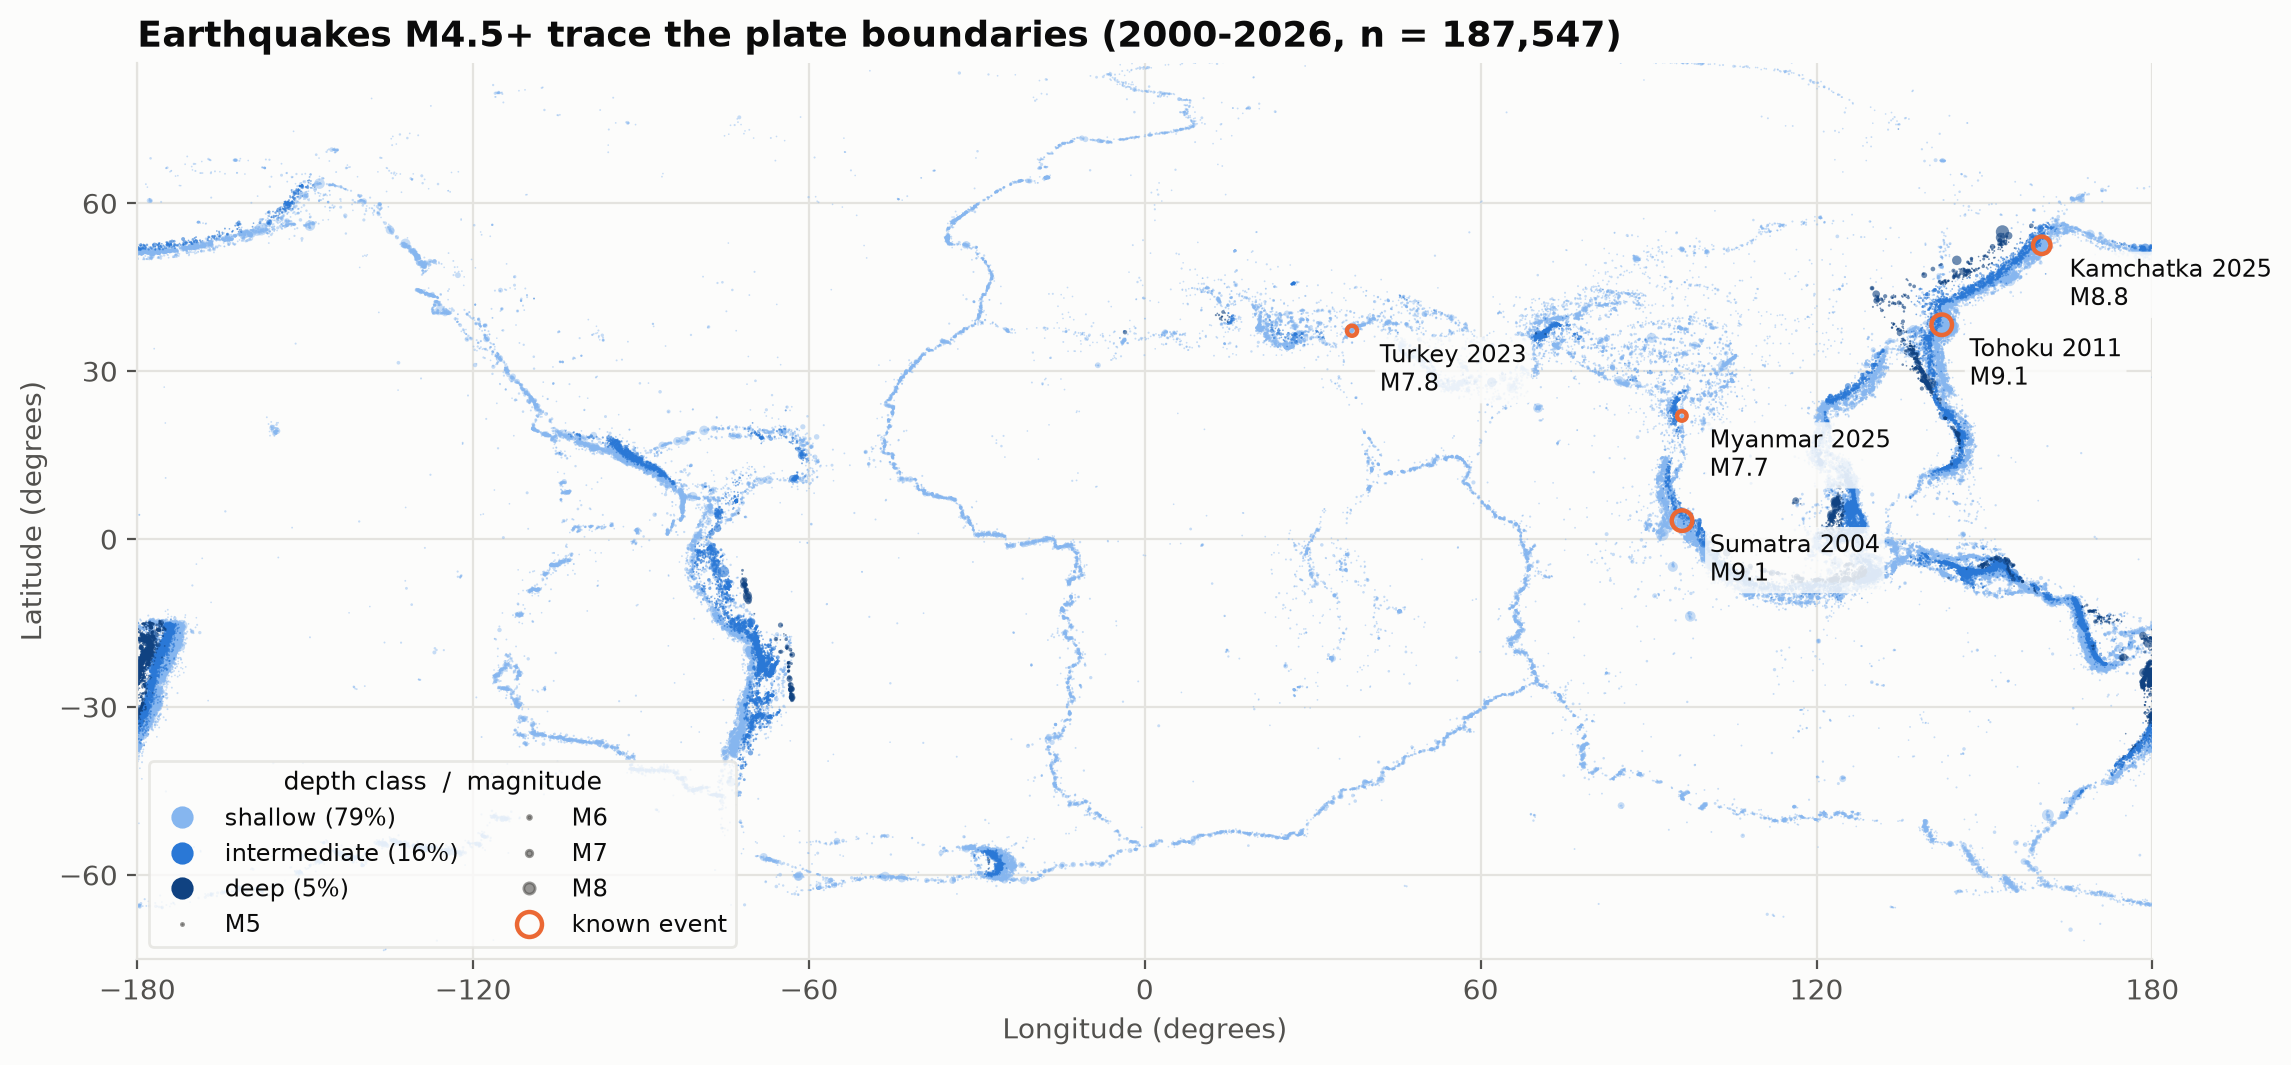
\includegraphics[width=\textwidth]{step4_world_map.png}
\caption{ตำแหน่งแผ่นดินไหว M4.5+ ปี 2000--2026 กระจุกตัวตามแนวรอยต่อแผ่นเปลือกโลก โดยเฉพาะวงแหวนแห่งไฟรอบมหาสมุทรแปซิฟิก}
\end{figure}

\begin{itemize}
  \item ปีที่สมบูรณ์ (2000--2025) มีแผ่นดินไหวเฉลี่ย 6{,}983 ครั้งต่อปี ปีที่มากที่สุดคือ 2011 (9{,}583 ครั้ง) และน้อยที่สุดคือ 2001 (4{,}679 ครั้ง)
  \item เดือนที่มากที่สุดคือ มี.ค. 2011 มี 2{,}400 ครั้ง โดย 82\% เกิดในญี่ปุ่น (aftershock ของ Tohoku M9.1) ยอดสูงอื่น ๆ ก็มาจาก aftershock ของเหตุใหญ่เช่นกัน เช่น ม.ค. 2005 (Sumatra) และ ก.ค. 2025 (Kamchatka)
  \item ขนาดที่ทำให้แคตตาล็อกสมบูรณ์ (Mc, วิธี maximum curvature $+0.2$ \cite{wiemer2000,woessner2005}) คือ 4.7 ค่า $b$ ของ Gutenberg--Richter \cite{gr1944} จากวิธี maximum likelihood ของ Aki \cite{aki1965} คือ 1.14 (standard error 0.003)
  \item แผ่นดินไหว M6.5 ขึ้นไปมี 1{,}218 ครั้ง ใหญ่ที่สุดคือ M9.1 (Sumatra 2004 และ Tohoku 2011)
\end{itemize}

\begin{figure}[H]
\centering
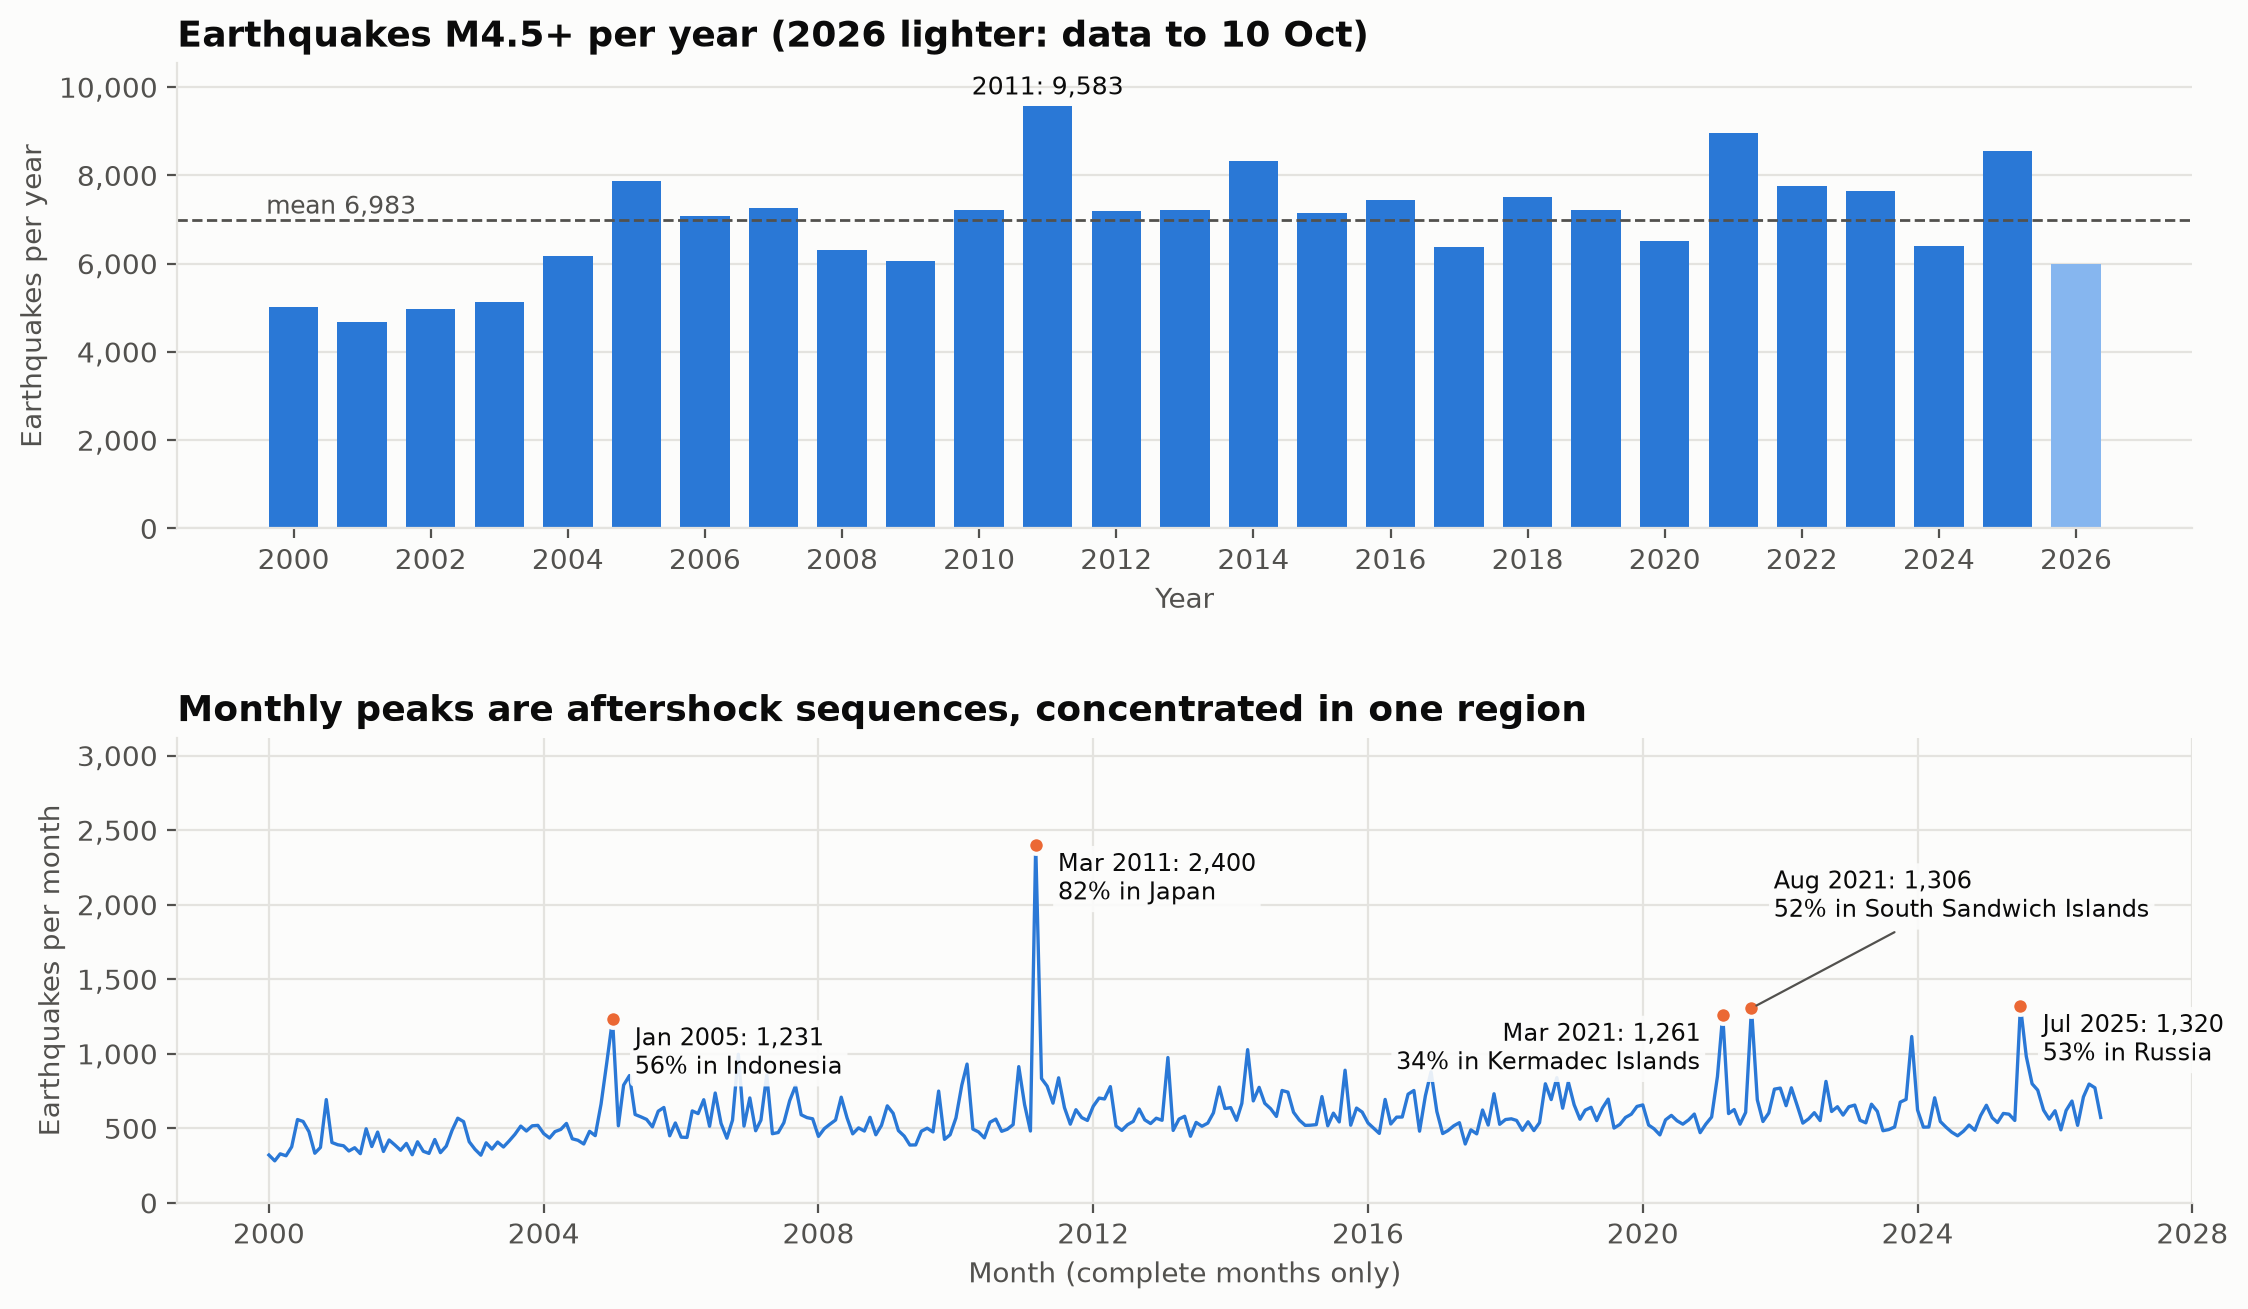
\includegraphics[width=0.49\textwidth]{step4_events_over_time.png}
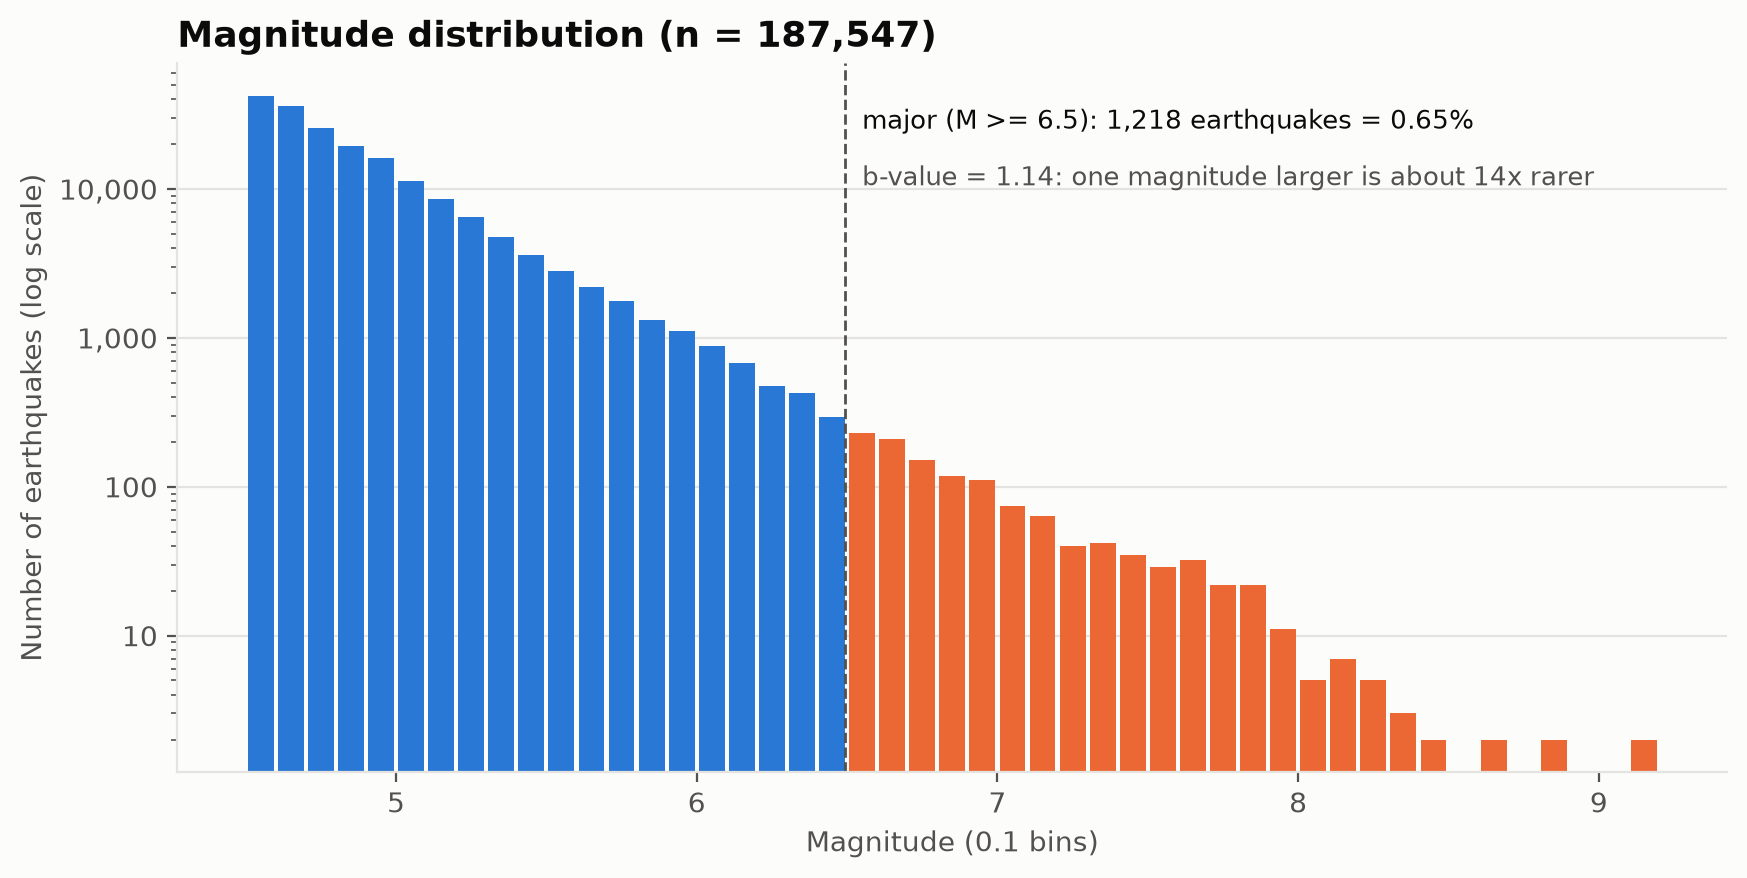
\includegraphics[width=0.49\textwidth]{step4_magnitude_hist.png}
\caption{ซ้าย: จำนวนแผ่นดินไหวรายเดือน ยอดแหลมคือช่วง aftershock ของเหตุใหญ่ \quad ขวา: การกระจายของขนาดแบบ log ลดลงเป็นเส้นตรงตามกฎ Gutenberg--Richter}
\end{figure}

\begin{figure}[H]
\centering
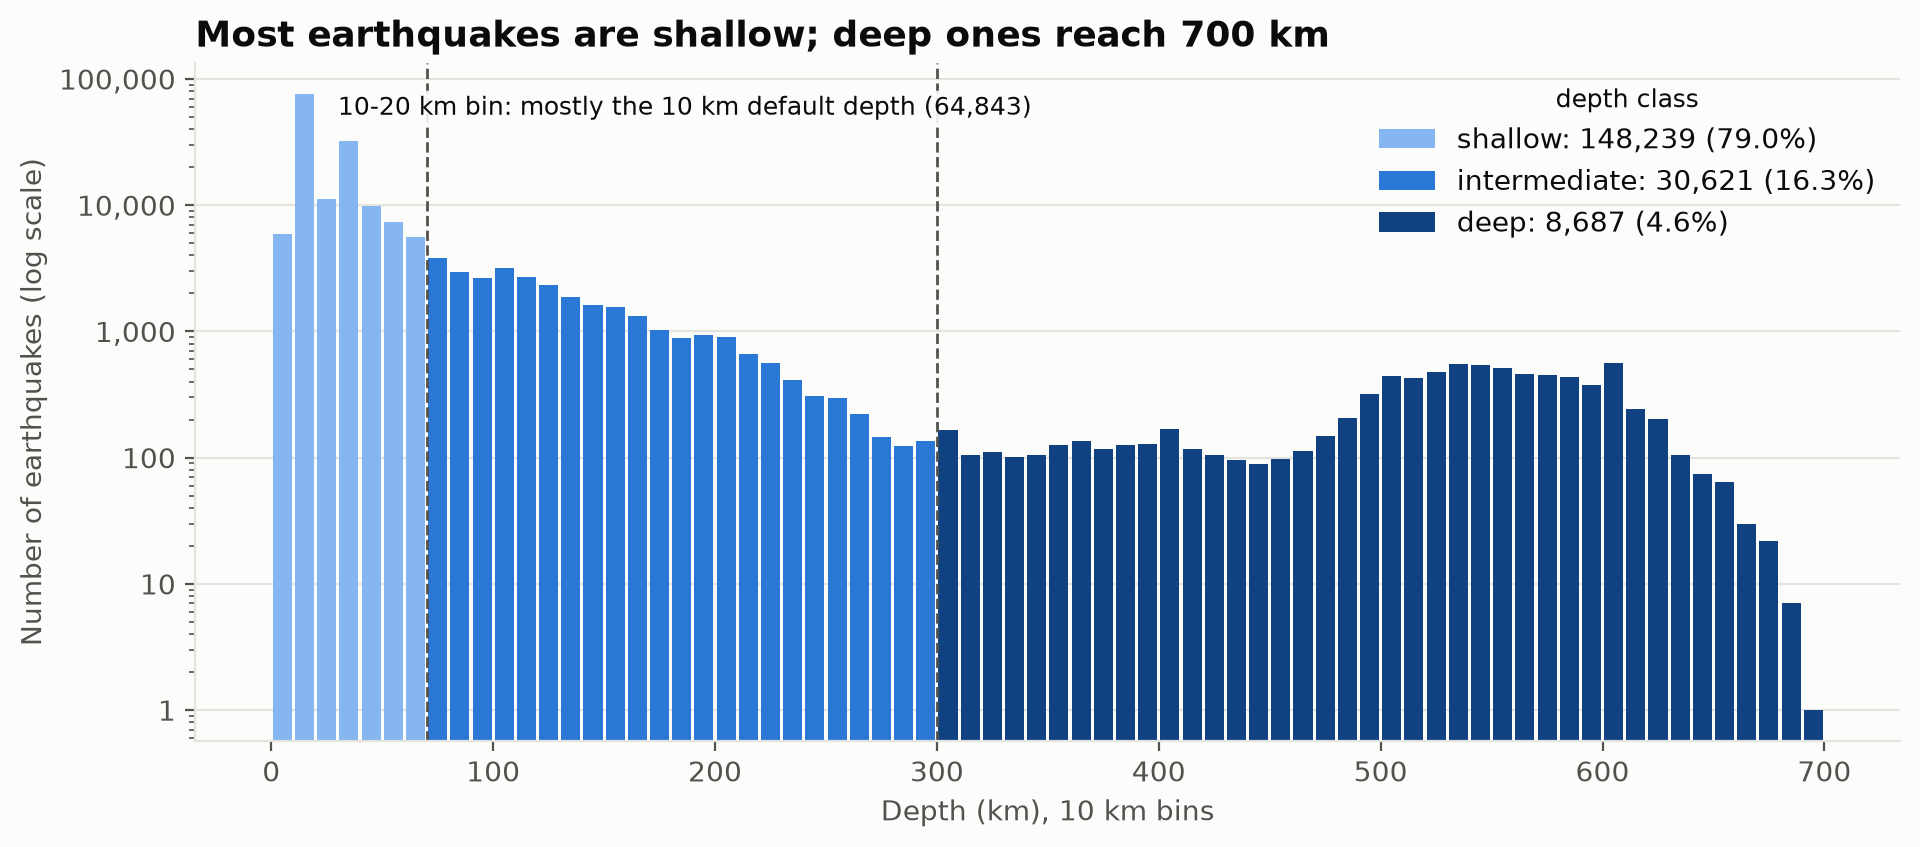
\includegraphics[width=0.49\textwidth]{step4_depth_hist.png}
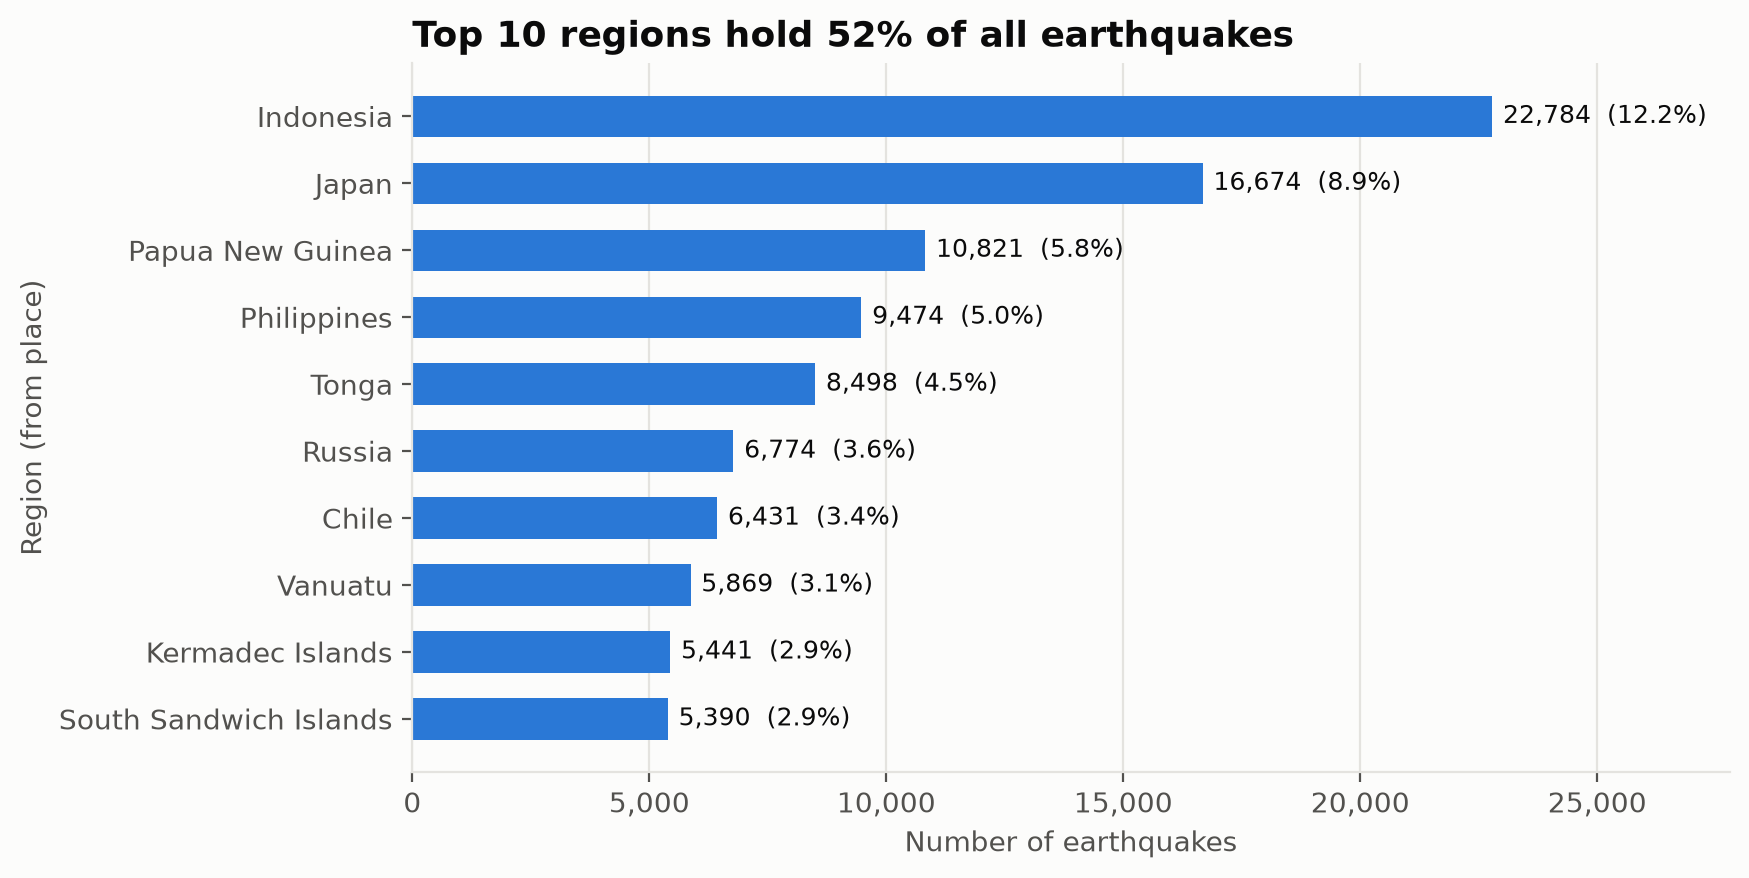
\includegraphics[width=0.49\textwidth]{step4_top_regions.png}
\caption{ซ้าย: การกระจายของความลึก มียอดแหลมที่ค่าซึ่งตั้งไว้ล่วงหน้า \quad ขวา: ภูมิภาคที่มีแผ่นดินไหวมากที่สุด}
\end{figure}

%======================================================================
\section{การเตรียมข้อมูล (Pre-processing)}
%======================================================================

\begin{figure}[H]
\centering
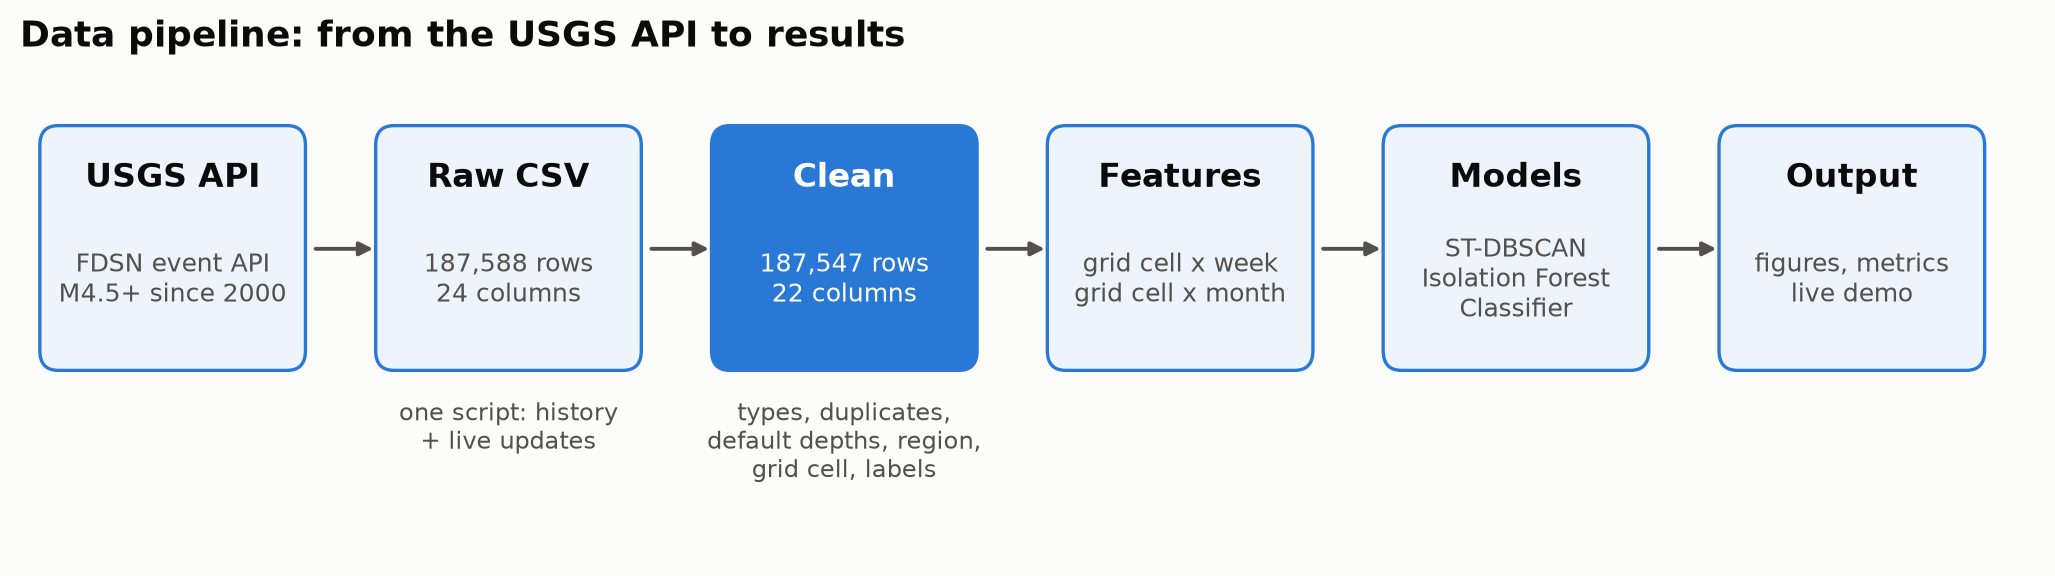
\includegraphics[width=\textwidth]{step3_pipeline.png}
\caption{ขั้นตอนการทำความสะอาดข้อมูล จาก 187{,}588 เหลือ 187{,}547 แถว}
\end{figure}

\begin{table}[H]
\centering\small
\begin{tabularx}{\textwidth}{@{}Xrr@{}}
\toprule
ขั้นตอน & แถวที่เหลือ & ตัดออก \\
\midrule
อ่านไฟล์ดิบ แปลงเวลาเป็น UTC & 187{,}588 & 0 \\
ตัดเหตุการณ์ที่ถูกลบ และที่ไม่ใช่ earthquake & 187{,}588 & 0 \\
ตัดขนาดต่ำกว่า 4.5 (ถูกปรับขนาดลงทีหลัง) & 187{,}584 & 4 \\
ตัดแถวที่ค่าหลักหาย & 187{,}584 & 0 \\
\code{id} ซ้ำ: เก็บแถวที่ \code{updated} ใหม่สุด & 187{,}584 & 0 \\
เหตุการณ์เดียวกันแต่มี 2 \code{id} ($\le 10$ วินาที และ $\le 10$ km): เก็บแถวที่ขนาดใหญ่กว่า & 187{,}547 & 37 \\
\midrule
\code{quakes\_clean.csv} \textbf{(22 คอลัมน์)} & \textbf{187{,}547} & \textbf{41} \\
\bottomrule
\end{tabularx}
\caption{จำนวนแถวในแต่ละขั้นของการทำความสะอาด (\code{results/step3\_summary.csv})}
\end{table}

\subsection{การจัดการเชิงพื้นที่และเวลา}
\begin{itemize}
  \item \textbf{เวลา:} แปลงเป็น UTC แล้วแยกคอลัมน์ปีและเดือน
  \item \textbf{ความลึกที่ตั้งไว้ล่วงหน้า:} หาค่าความลึกที่มีจำนวนแถวมากกว่าค่ามัธยฐานของค่าข้างเคียงอย่างน้อย 10 เท่า และมีอย่างน้อย 1{,}000 แถว ได้ 4 ค่า (10, 30, 33, 35 km) รวม 87{,}087 แถว (46.4\%) เราไม่ลบแถวเหล่านี้ แต่ติดธง \code{depth\_fixed} ไว้
  \item \textbf{กลุ่มความลึก:} ตื้น (0--70 km), กลาง (70--300 km), ลึก (300 km ขึ้นไป)
  \item \textbf{ช่องตาราง:} แบ่งโลกเป็นช่องขนาด $5^\circ \times 5^\circ$ (\code{cell\_id}) มี 1{,}206 ช่องที่มีแผ่นดินไหว
  \item \textbf{ภูมิภาค:} ตัดข้อความหลังจุลภาคตัวสุดท้ายของ \code{place} ได้ 439 ภูมิภาค
  \item \textbf{ป้ายกำกับ:} \code{is\_major} = ขนาด 6.5 ขึ้นไป (1{,}218 แถว, 0.65\%)
\end{itemize}

\begin{figure}[H]
\centering
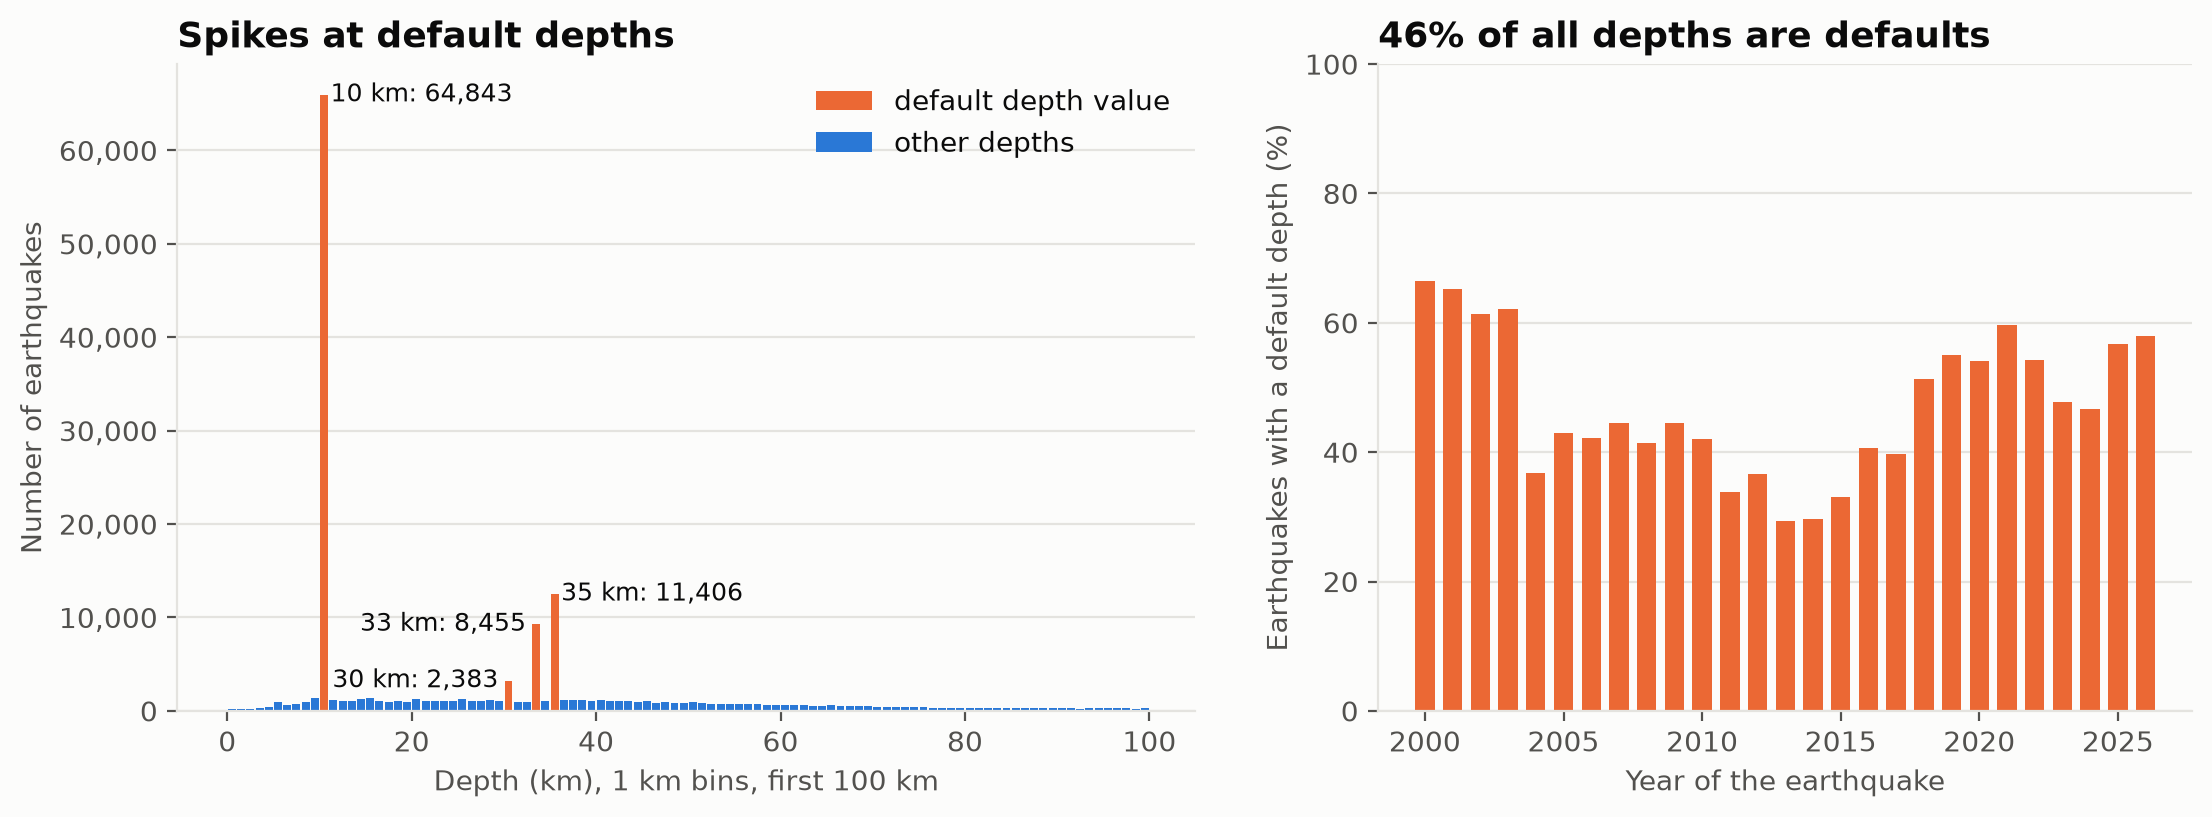
\includegraphics[width=0.49\textwidth]{step3_depth_fixed.png}
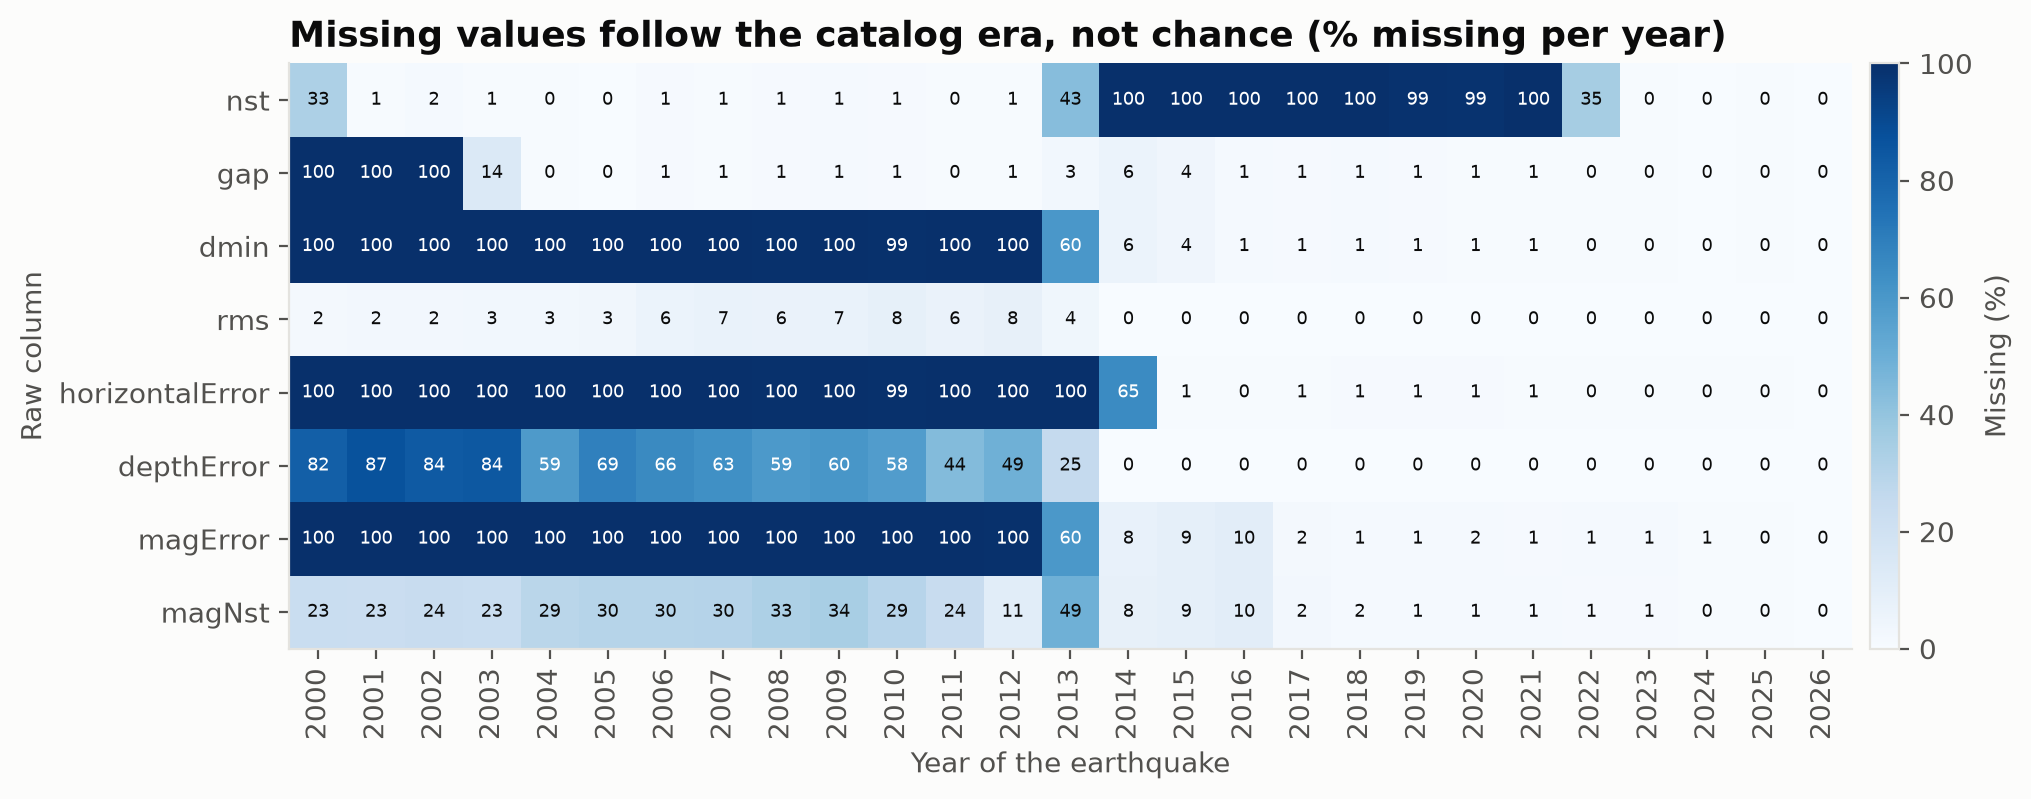
\includegraphics[width=0.49\textwidth]{step3_missing_by_year.png}
\caption{ซ้าย: ค่าความลึกที่ตั้งไว้ล่วงหน้า \quad ขวา: \% ค่าว่างของคอลัมน์คุณภาพในแต่ละปี ค่าว่างขึ้นกับยุคของแคตตาล็อก ไม่ได้หายแบบสุ่ม เราจึงไม่ใช้คอลัมน์เหล่านี้เป็น feature}
\end{figure}

%======================================================================
\section{เทคนิคการวิเคราะห์}
%======================================================================

ทุกเทคนิคแบ่งข้อมูลตามเวลา ไม่แบ่งแบบสุ่ม: ฝึกด้วยปี 2000--2019, เลือกค่าด้วยปี 2020--2022,
และวัดผลจริงด้วยปี 2023 เป็นต้นไป ซึ่งโมเดลไม่เคยเห็นมาก่อน

\subsection{ST-DBSCAN: จับกลุ่ม aftershock และ swarm}
DBSCAN \cite{ester1996} ใช้ระยะทางอย่างเดียว ST-DBSCAN \cite{birant2007} เพิ่มเงื่อนไขเวลา
สองเหตุการณ์จะเป็นเพื่อนบ้านกันเมื่ออยู่ห่างกันไม่เกิน $\varepsilon_1$ km \textbf{และ}เกิดห่างกันไม่เกิน $\varepsilon_2$ วัน

ไลบรารี \code{st-dbscan} ติดตั้งบน Python 3.14 ไม่ได้ เราจึงเขียนเอง โดยใช้ KD-tree หาคู่ที่อาจเป็นเพื่อนบ้าน
แล้วกรองด้วยระยะ haversine จริงกับช่วงเวลา สร้างเป็นกราฟแบบ sparse แล้วส่งให้ \code{DBSCAN(metric="precomputed")}
ของ scikit-learn \cite{sklearn}

\textbf{การเลือกค่า:} กราฟ k-distance (ระยะไปยังเพื่อนบ้านลำดับที่ 4 ภายใน 7 วัน) มีจุดหักโค้ง (Kneedle \cite{satopaa2011}) ที่ 38 km
แต่ค่านี้เป็นแค่ขอบล่าง เพราะรอยเลื่อนของเหตุใหญ่ยาวหลายร้อยกิโลเมตร (Sumatra 2004 ยาวราว 1{,}300 km)
เราจึงลองทุกชุดของ $\varepsilon_1 \in \{25, 50, 100, 150\}$ km, $\varepsilon_2 \in \{3, 7, 14, 30\}$ วัน, min\_samples $\in \{5, 10\}$
แล้วดูว่าจับ aftershock ของเหตุการณ์ใหญ่ที่รู้จัก 5 เหตุการณ์ได้ดีแค่ไหน โดยไม่ให้กลุ่มลากยาวจนผิดธรรมชาติ
ค่าที่เลือกคือ $\varepsilon_1 = 100$ km, $\varepsilon_2 = 7$ วัน, min\_samples $= 5$
ที่ 7 วันและ min\_samples 5 สัดส่วน aftershock ของ Sumatra ที่จับได้คือ 0.00 ที่ 25 km, 0.86 ที่ 50 km และ 0.98 ที่ 100 km
ส่วนที่ 150 km กลุ่มเริ่มเชื่อมต่อกันยาวถึง 488 วัน

แต่ละกลุ่มถูกแบ่งเป็น \textbf{aftershock sequence} (เหตุการณ์ที่เกิดก่อน mainshock ไม่เกิน 20\%) หรือ \textbf{swarm} (เกิน 20\%)

\begin{figure}[H]
\centering
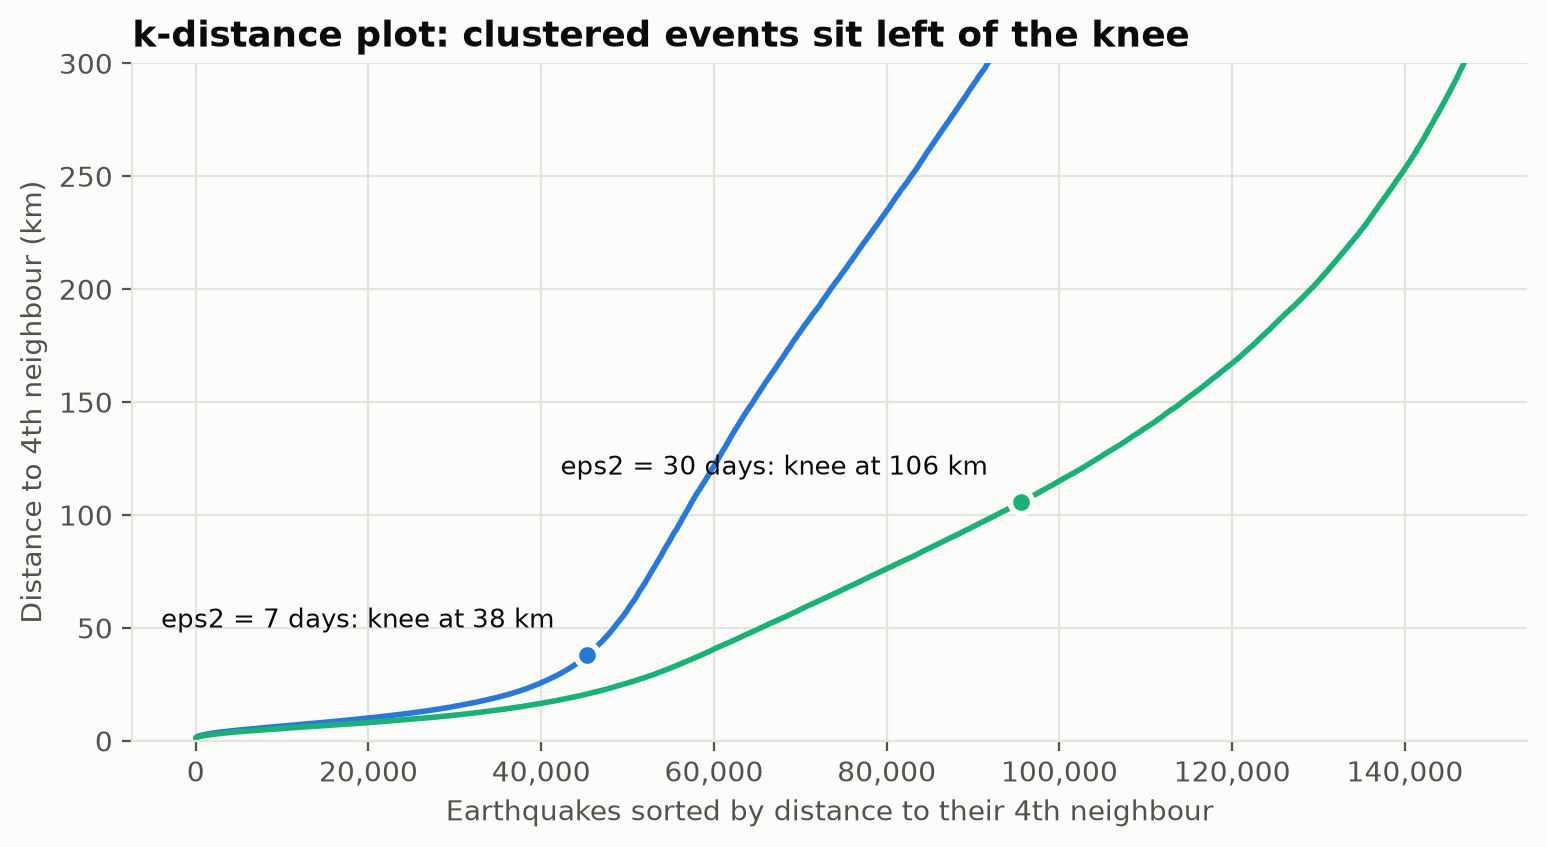
\includegraphics[width=0.49\textwidth]{step5_kdistance.png}
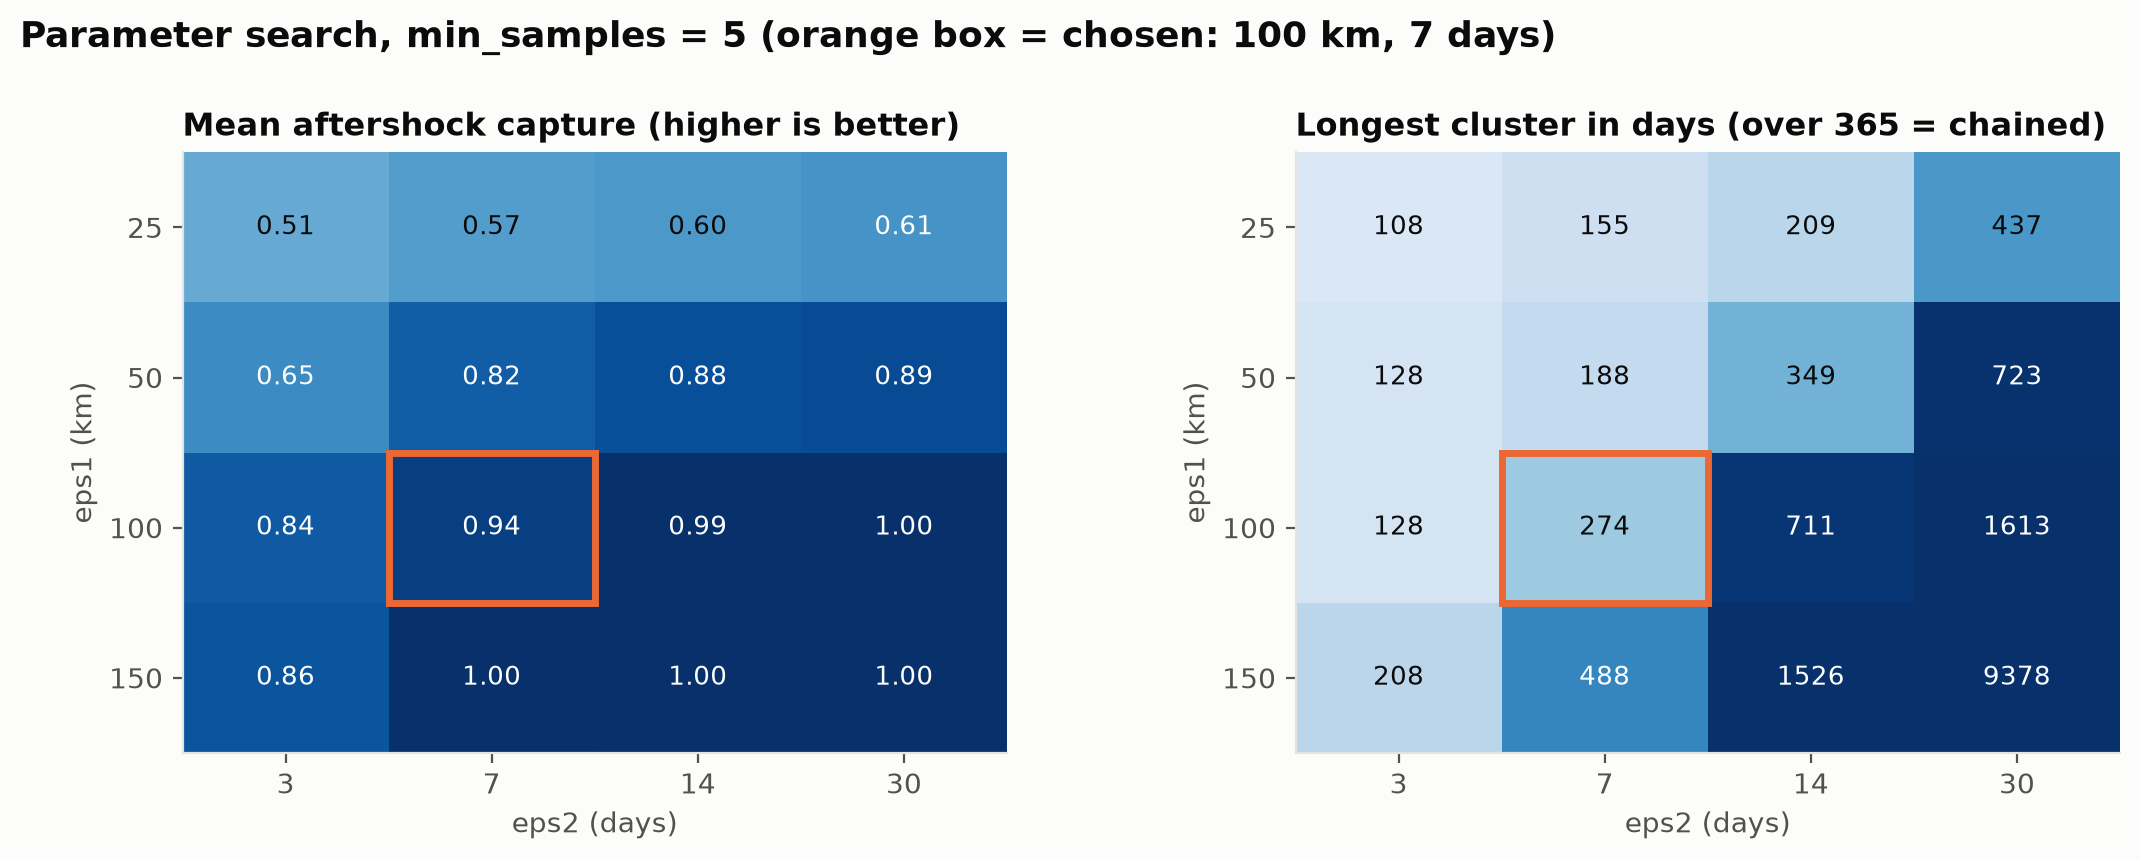
\includegraphics[width=0.49\textwidth]{step5_param_search.png}
\caption{ซ้าย: กราฟ k-distance \quad ขวา: ผลการลองค่า $\varepsilon_1$, $\varepsilon_2$}
\end{figure}

\subsection{Isolation Forest: หาช่องตาราง-สัปดาห์ที่ผิดปกติ}
Isolation Forest \cite{liu2008} แยกจุดข้อมูลด้วยการตัดแบบสุ่ม จุดที่ผิดปกติจะถูกแยกออกได้เร็ว (ความลึกของต้นไม้น้อย)
หน่วยของข้อมูลคือ \textbf{ช่องตาราง $\times$ สัปดาห์} ที่มีแผ่นดินไหวอย่างน้อย 1 ครั้ง (91{,}350 แถว)
feature ได้แก่ จำนวนเหตุการณ์ (\code{n\_events}), log ของอัตราเทียบกับค่าปกติของช่องนั้น (\code{log\_rate\_ratio}, ค่าปกติคิดจากปี 2000--2019 เท่านั้น),
ความลึกเฉลี่ย, ระยะกระจายจากจุดศูนย์กลาง (\code{spread\_km}) และขนาดเฉลี่ย ใช้ต้นไม้ 300 ต้น

โมเดลนี้เรียนรู้แบบไม่มีป้ายกำกับ แต่เพื่อวัดผลได้ เรากำหนดว่าช่อง-สัปดาห์ที่มีแผ่นดินไหว M7.0 ขึ้นไปคือความผิดปกติจริง
เพื่อทดสอบ leakage เราฝึก 3 ชุด
\textbf{A} ใช้ขนาดสูงสุดด้วย (ซึ่งคำนวณจากค่าเดียวกับคำตอบ),
\textbf{B} ไม่ใช้ขนาดสูงสุด (ผลที่ซื่อตรง และเป็นโมเดลที่ใช้ใน live demo),
\textbf{C} ไม่ใช้ข้อมูลขนาดเลย
ค่า contamination 0.002 เลือกจากชุด validation (F1 สูงสุดของชุด B)

\subsection{Imbalanced classification: ทำนายแผ่นดินไหวใหญ่เดือนถัดไป}
หน่วยของข้อมูลคือ \textbf{ช่องตาราง $\times$ เดือน} (1{,}204 ช่อง $\times$ 320 เดือน) เป้าหมาย $y = 1$
ถ้าเดือนถัดไปมีแผ่นดินไหว M6.5 ขึ้นไปในช่องนั้น feature 15 ตัวใช้ข้อมูลถึงเดือนปัจจุบันเท่านั้น
เช่น จำนวนเหตุการณ์ย้อนหลัง 1/3/12 เดือน, จำนวนแผ่นดินไหวใหญ่ 12 เดือน, จำนวนเดือนนับจากแผ่นดินไหวใหญ่ครั้งล่าสุด,
สัดส่วนความลึก และกิจกรรมของช่องข้างเคียง

\begin{figure}[H]
\centering
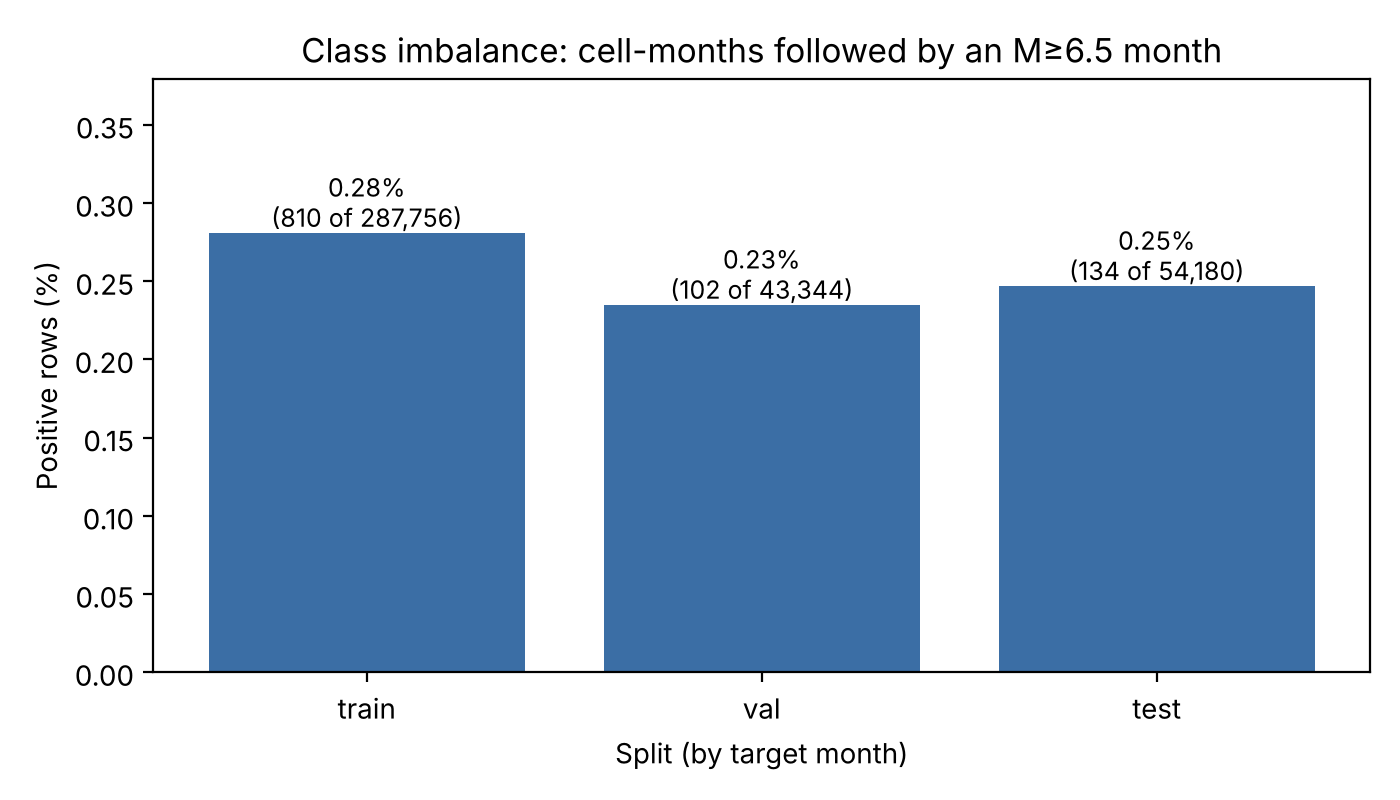
\includegraphics[width=0.6\textwidth]{step7_class_balance.png}
\caption{สัดส่วนคลาสบวกในแต่ละช่วง (ประมาณ 0.25\%, 1 ต่อ 400)}
\end{figure}

\textbf{การป้องกัน leakage} (ผ่านทั้ง 8 ข้อ, \code{results/step7\_leakage\_checks.csv}):
สร้าง feature ใหม่โดยตัดข้อมูลหลังเดือน 2010-06, 2019-12 และ 2023-03 แล้วค่าต้องไม่เปลี่ยน,
คำนวณ $y$ ใหม่จากเหตุการณ์จริง, ตรวจว่าป้ายของ train ไม่เลยปี 2019, และไม่ใช้คอลัมน์คุณภาพรายเหตุการณ์
เช่น \code{magType} หรือ \code{nst}

\textbf{โมเดลที่เทียบ:}
\begin{enumerate}
  \setcounter{enumi}{-1}
  \item Naive baseline: ทายว่าเป็นบวกถ้าช่องนั้นมีแผ่นดินไหวใหญ่ใน 12 เดือนที่ผ่านมา
  \item Logistic Regression ไม่จัดการความไม่สมดุล
  \item Logistic Regression + \code{class\_weight="balanced"}
  \item LightGBM \cite{ke2017} + class weight
  \item LightGBM + SMOTE \cite{chawla2002} (ทำบน train เท่านั้น ให้คลาสบวกเป็น 10\%)
  \item โมเดลที่ PR-AUC บน validation ดีที่สุด + threshold ที่ปรับให้ F1 บน validation สูงสุด
\end{enumerate}
feature แบบนับจำนวนเบ้มาก จึงแปลงด้วย \code{log1p} และ standardise ก่อนเข้า Logistic Regression
ส่วนค่าตั้งของ LightGBM เลือกจาก grid 12 ชุดโดยดู PR-AUC บน validation เท่านั้น ชุด test ใช้แค่ครั้งเดียวตอนท้าย

%======================================================================
\section{การประเมินผลและผลลัพธ์}
%======================================================================

\subsection{ST-DBSCAN}
\begin{itemize}
  \item ได้ 3{,}567 กลุ่ม (aftershock sequence 1{,}991, swarm 1{,}576) มี 1{,}127 กลุ่มที่มี 10 เหตุการณ์ขึ้นไป
  \item 66.5\% ของเหตุการณ์เป็น noise (ไม่อยู่ในกลุ่มใด) ส่วนแผ่นดินไหวใหญ่อยู่ในกลุ่ม 63.4\%
  \item เหตุการณ์ใหญ่ที่รู้จัก 5 เหตุการณ์อยู่ในกลุ่มครบทั้ง 5 จับ aftershock ได้เฉลี่ย 0.94 (ตารางที่ \ref{tab:known})
  \item กลุ่มใหญ่ที่สุด 3 อันดับคือ Tohoku 2011 (2{,}980 เหตุการณ์, 215 วัน), Sumatra 2004 (2{,}326, 274 วัน) และ Kamchatka 2025 (1{,}681, 142 วัน)
\end{itemize}

\begin{table}[H]
\centering\small
\begin{tabular}{@{}lrrrr@{}}
\toprule
เหตุการณ์ & ขนาด & อันดับกลุ่ม & เหตุการณ์ในกลุ่ม & สัดส่วนที่จับได้ \\
\midrule
Sumatra 2004 & 9.1 & 2 & 2{,}326 & 0.98 \\
Tohoku 2011 & 9.1 & 1 & 2{,}980 & 1.00 \\
Turkey 2023 & 7.8 & 49 & 154 & 0.91 \\
Myanmar 2025 & 7.7 & 448 & 20 & 0.82 \\
Kamchatka 2025 & 8.8 & 3 & 1{,}681 & 1.00 \\
\bottomrule
\end{tabular}
\caption{ตรวจกลุ่มกับเหตุการณ์จริง สัดส่วนที่จับได้ = aftershock ใน 30 วันและ 300 km ที่อยู่ในกลุ่มเดียวกับ mainshock (\code{results/step5\_known\_events\_check.csv})}
\label{tab:known}
\end{table}

\begin{figure}[H]
\centering
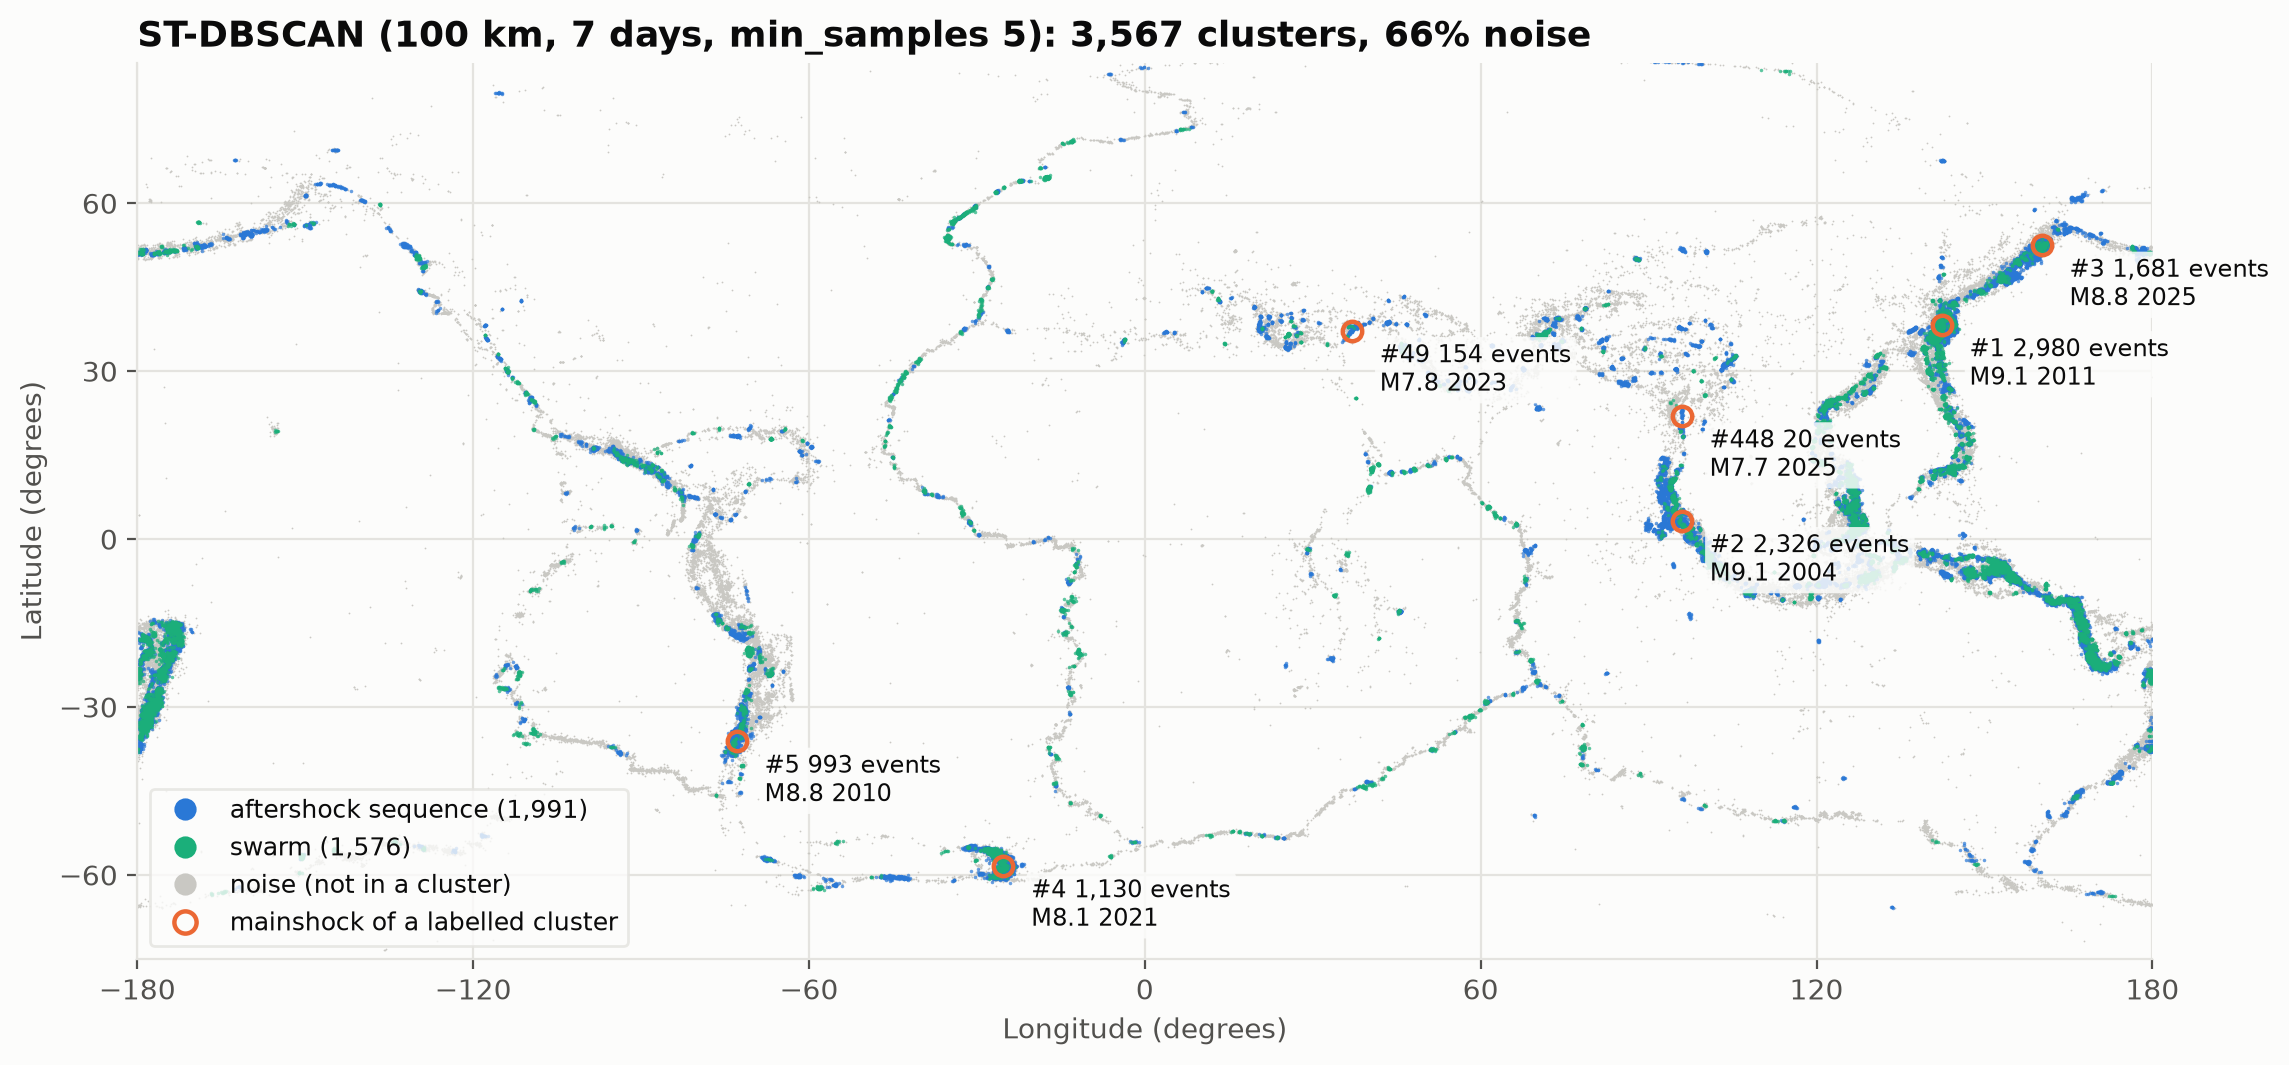
\includegraphics[width=\textwidth]{step5_clusters_map.png}
\caption{แผนที่กลุ่มจาก ST-DBSCAN สีน้ำเงิน = aftershock sequence, สีเขียว = swarm, สีเทา = noise}
\end{figure}

\begin{figure}[H]
\centering
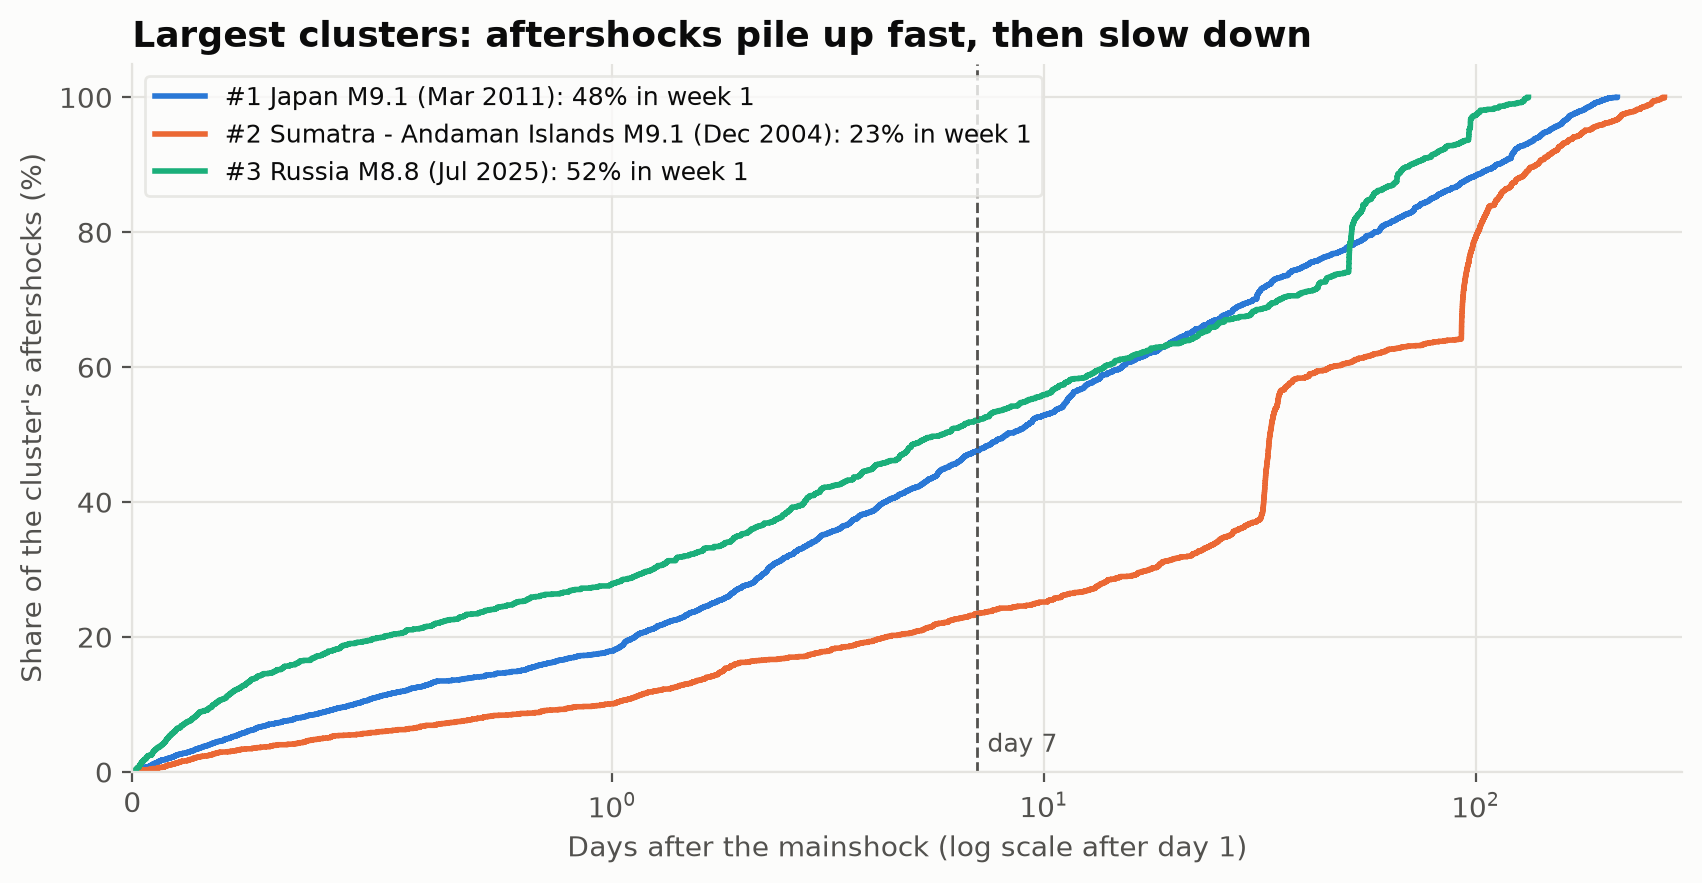
\includegraphics[width=0.85\textwidth]{step5_top_clusters.png}
\caption{กลุ่มใหญ่ที่สุด จำนวน aftershock ลดลงตามเวลาตามกฎของ Omori \cite{utsu1995}}
\end{figure}

\subsection{Isolation Forest}
ชุด test (ปี 2023 เป็นต้นไป) มี 13{,}548 ช่อง-สัปดาห์ เป็นความผิดปกติจริง 54 แถว
การเดาสุ่มได้ precision 0.004

\begin{table}[H]
\centering\small
\resizebox{\textwidth}{!}{%
\begin{tabular}{@{}lrrrrr@{}}
\toprule
ชุด feature & Precision & Recall & F1 & PR-AUC & เทียบการเดาสุ่ม \\
\midrule
A: มีขนาดสูงสุด (leakage) & 0.759 & 0.407 & 0.530 & 0.601 & 190 เท่า \\
\textbf{B: ไม่มีขนาดสูงสุด} & \textbf{0.424} & \textbf{0.259} & \textbf{0.322} & \textbf{0.274} & \textbf{106 เท่า} \\
C: ไม่ใช้ขนาดเลย & 0.485 & 0.296 & 0.368 & 0.244 & 122 เท่า \\
\bottomrule
\end{tabular}}
\caption{ผล Isolation Forest บนชุด test ที่ contamination 0.002 (\code{results/anomaly\_metrics.csv})}
\end{table}

ช่องว่างระหว่างชุด A กับ B คือผลของ leakage: ถ้าใส่ขนาดสูงสุดซึ่งคำนวณจากค่าเดียวกับคำตอบ ผลจะดูดีเกินจริง
ชุด B และ C ยังดีกว่าการเดาสุ่มกว่า 100 เท่า แสดงว่ากิจกรรมที่สูงผิดปกติ (จำนวนและอัตราเทียบกับค่าปกติ)
สัมพันธ์กับการเกิดแผ่นดินไหวใหญ่จริง แต่ feature คิดจากสัปดาห์เดียวกับเหตุใหญ่ ซึ่งรวม aftershock ของเหตุนั้นด้วย
ผลนี้จึงเป็นการ\textbf{ตรวจจับ}ไม่ใช่การ\textbf{ทำนายล่วงหน้า}

\begin{figure}[H]
\centering
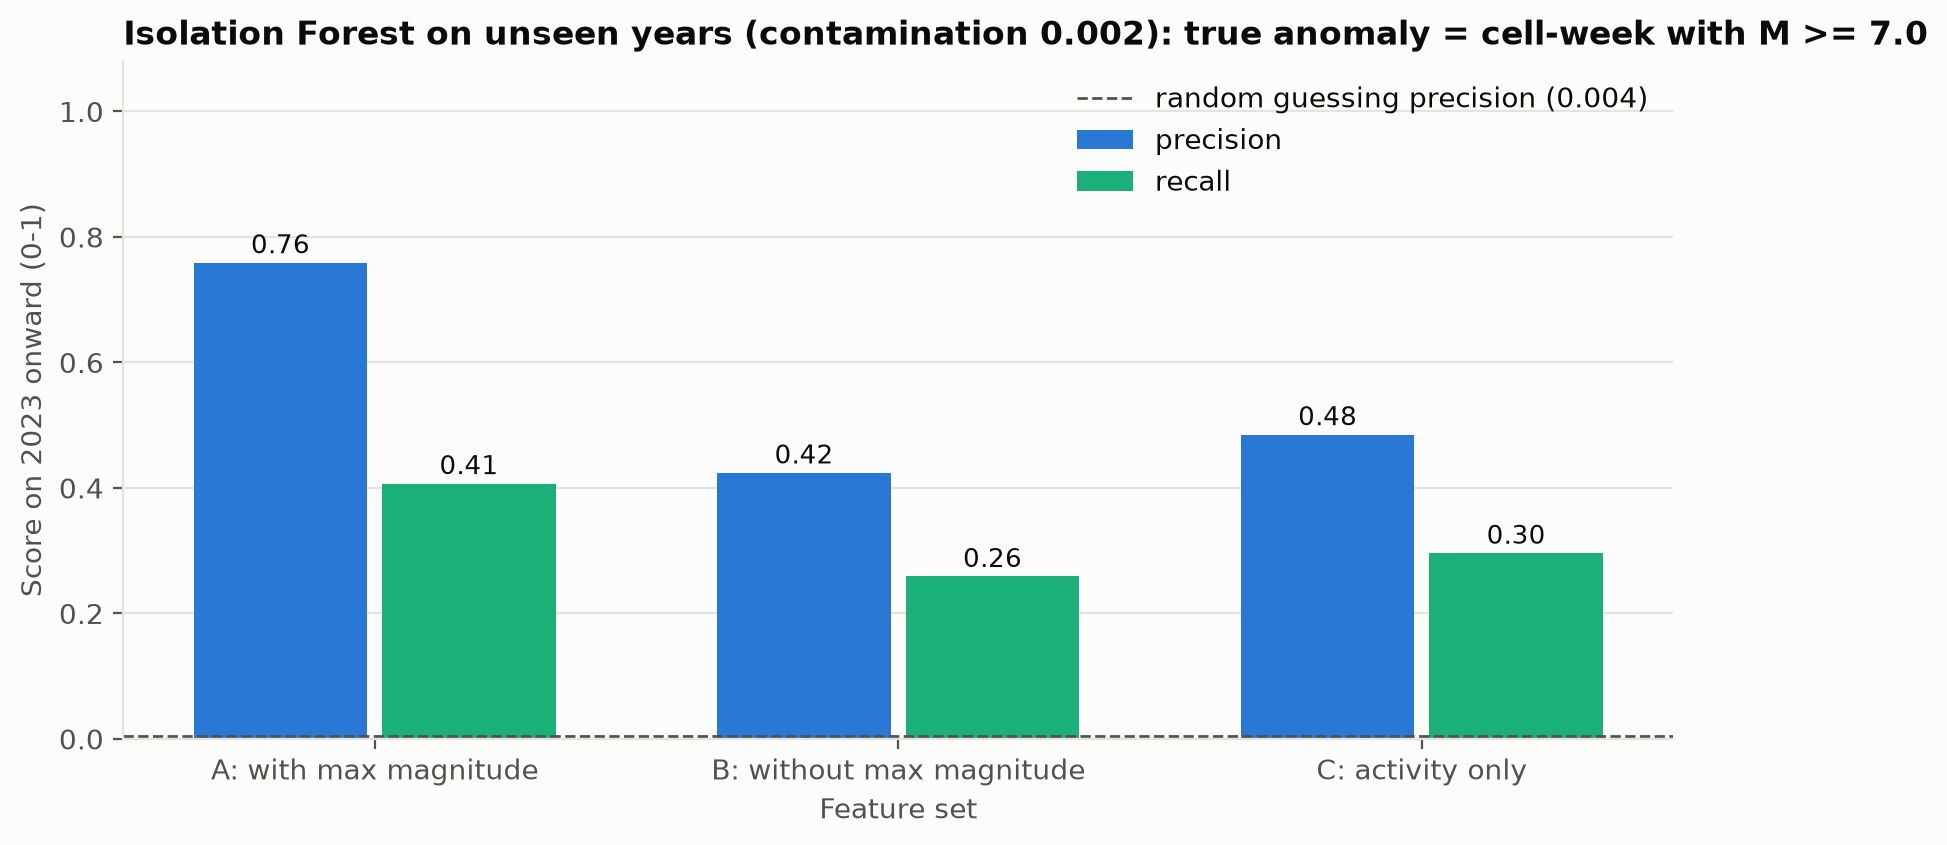
\includegraphics[width=0.49\textwidth]{step6_metrics.png}
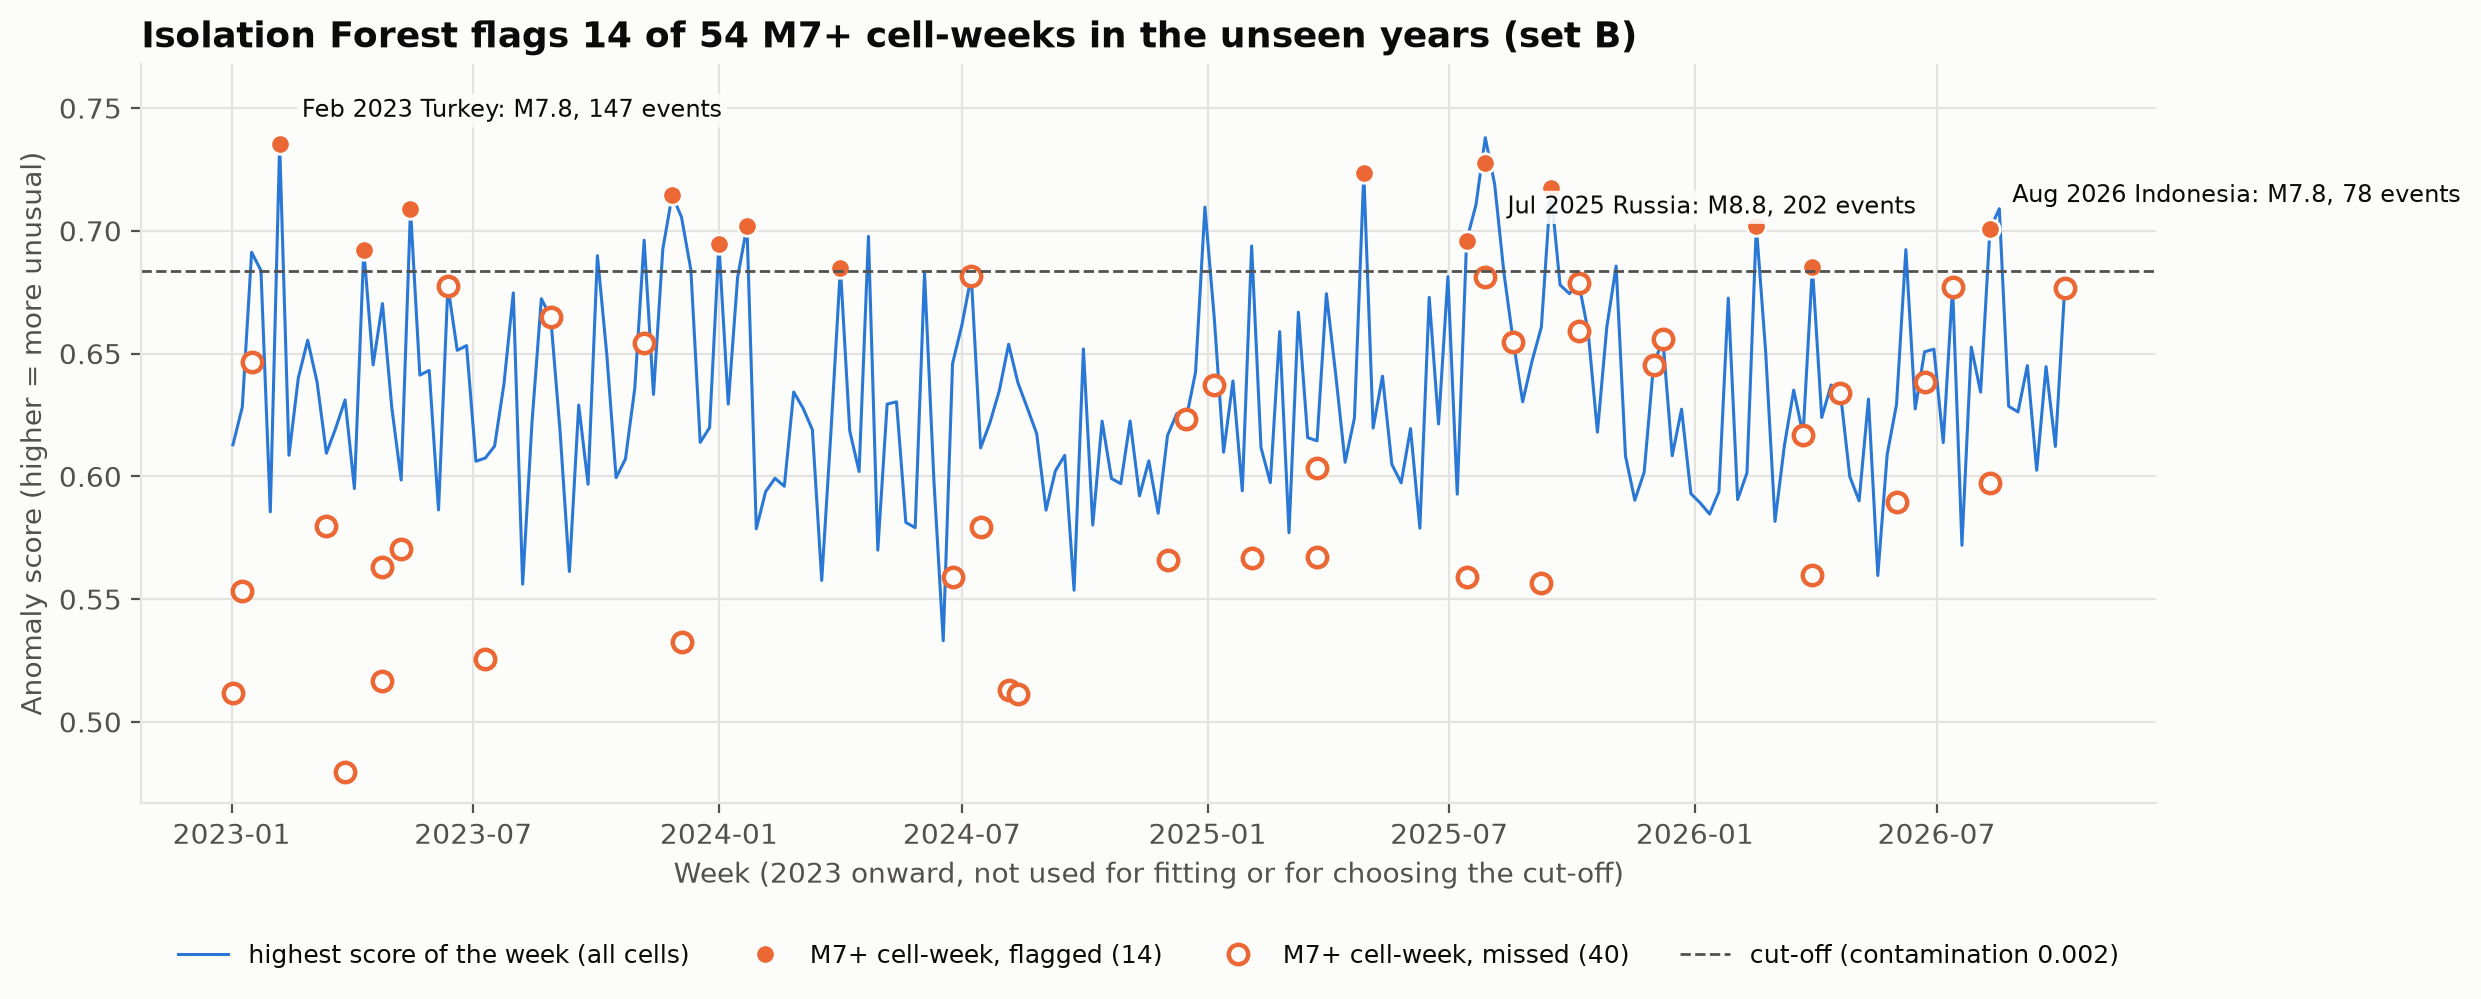
\includegraphics[width=0.49\textwidth]{step6_anomaly_timeline.png}
\caption{ซ้าย: ผลของ 3 ชุด feature ที่ค่า contamination ต่าง ๆ \quad ขวา: ช่อง-สัปดาห์ที่ถูก flag ตามเวลา}
\end{figure}

\subsection{Imbalanced classification}
ชุด test มี 54{,}180 แถว เป็นบวก 134 แถว (0.25\%) การเดาสุ่มได้ PR-AUC 0.0025

\begin{table}[H]
\centering\small
\resizebox{\textwidth}{!}{%
\begin{tabular}{@{}lrrrrr@{}}
\toprule
โมเดล (threshold จาก validation) & Threshold & Precision & Recall & F1 & PR-AUC \\
\midrule
0. Naive baseline & กฎ & 0.023 & 0.239 & 0.043 & 0.012 \\
1. Logistic Regression & 0.086 & 0.048 & 0.060 & 0.053 & 0.043 \\
\textbf{2/5. Logistic Regression + class weight} & \textbf{0.972} & \textbf{0.055} & \textbf{0.142} & \textbf{0.079} & \textbf{0.041} \\
3. LightGBM + class weight & 0.952 & 0.054 & 0.090 & 0.067 & 0.035 \\
4. LightGBM + SMOTE & 0.544 & 0.043 & 0.119 & 0.063 & 0.029 \\
\bottomrule
\end{tabular}}
\caption{ผลบนชุด test เมื่อทุกโมเดลได้ threshold ที่ปรับบน validation (\code{results/step8\_tuned\_threshold\_comparison.csv}, \code{classification\_metrics.csv})}
\end{table}

\begin{itemize}
  \item \textbf{Accuracy ใช้ไม่ได้:} Logistic Regression ที่ threshold 0.5 ไม่จัดการความไม่สมดุลได้ accuracy 99.75\% แต่จับแผ่นดินไหวใหญ่ได้ 0 จาก 134 เราจึงใช้ precision, recall, F1 และ PR-AUC แทน \cite{saito2015}
  \item \textbf{โมเดลที่ดีที่สุด} คือ Logistic Regression + class weight ที่ threshold 0.972 ได้ precision 0.055, recall 0.142, F1 0.079, PR-AUC 0.041 (16 เท่าของการเดาสุ่ม)
  \item \textbf{ชนะ baseline อย่างมีนัยสำคัญ:} bootstrap 2{,}000 รอบ (สุ่มทีละเดือนทั้งเดือน) ได้ F1 ดีกว่า $+0.037$ (95\% CI $+0.013$ ถึง $+0.061$) และ PR-AUC ดีกว่า $+0.029$ (95\% CI $+0.010$ ถึง $+0.052$)
  \item \textbf{ยังไม่ใช่ระบบเตือนภัย:} มี false alarm 326 จาก 345 ครั้งที่เตือน และพลาด 115 จาก 134 เหตุการณ์
  \item \textbf{LightGBM ไม่ช่วย:} โมเดลที่ซับซ้อนกว่าไม่ชนะ เพราะสัญญาณอ่อนและมีตัวอย่างบวกใน validation แค่ 102 ตัว
  \item \textbf{Feature ที่มีผลชัด} คือ \code{n\_major\_12m} และ \code{nbr\_major\_12m} คือกิจกรรมแผ่นดินไหวใหญ่ล่าสุดในช่องนั้นและช่องข้างเคียง
\end{itemize}

\begin{figure}[H]
\centering
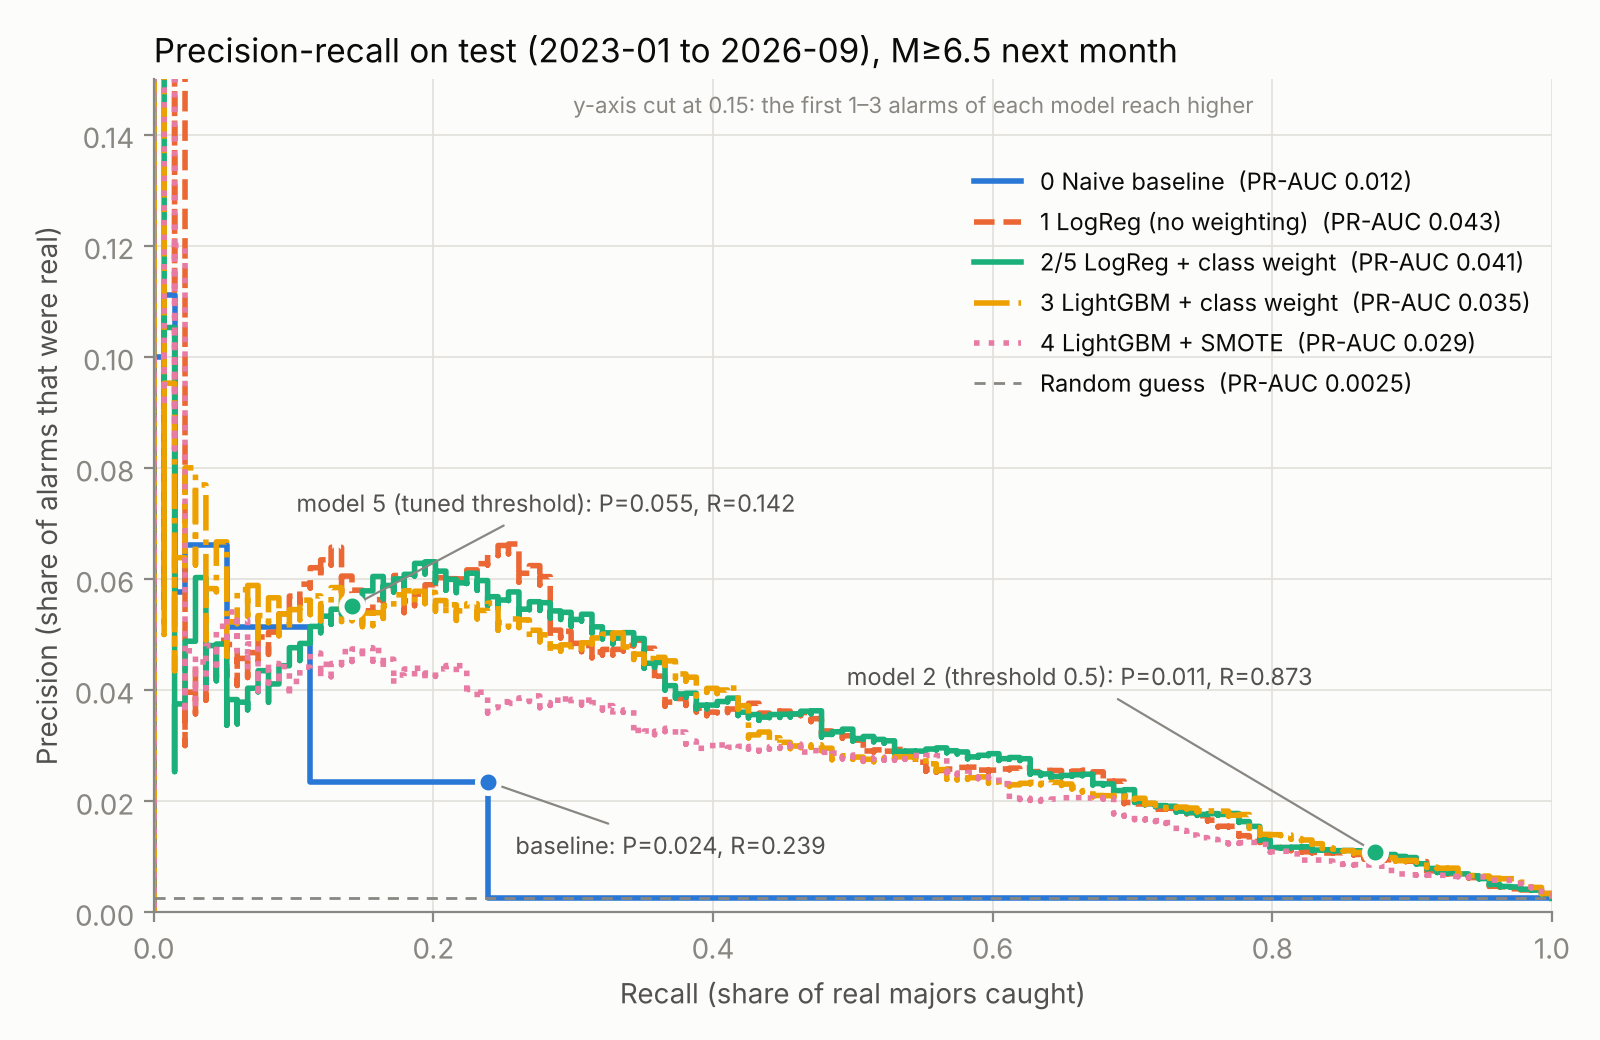
\includegraphics[width=0.49\textwidth]{step9_pr.png}
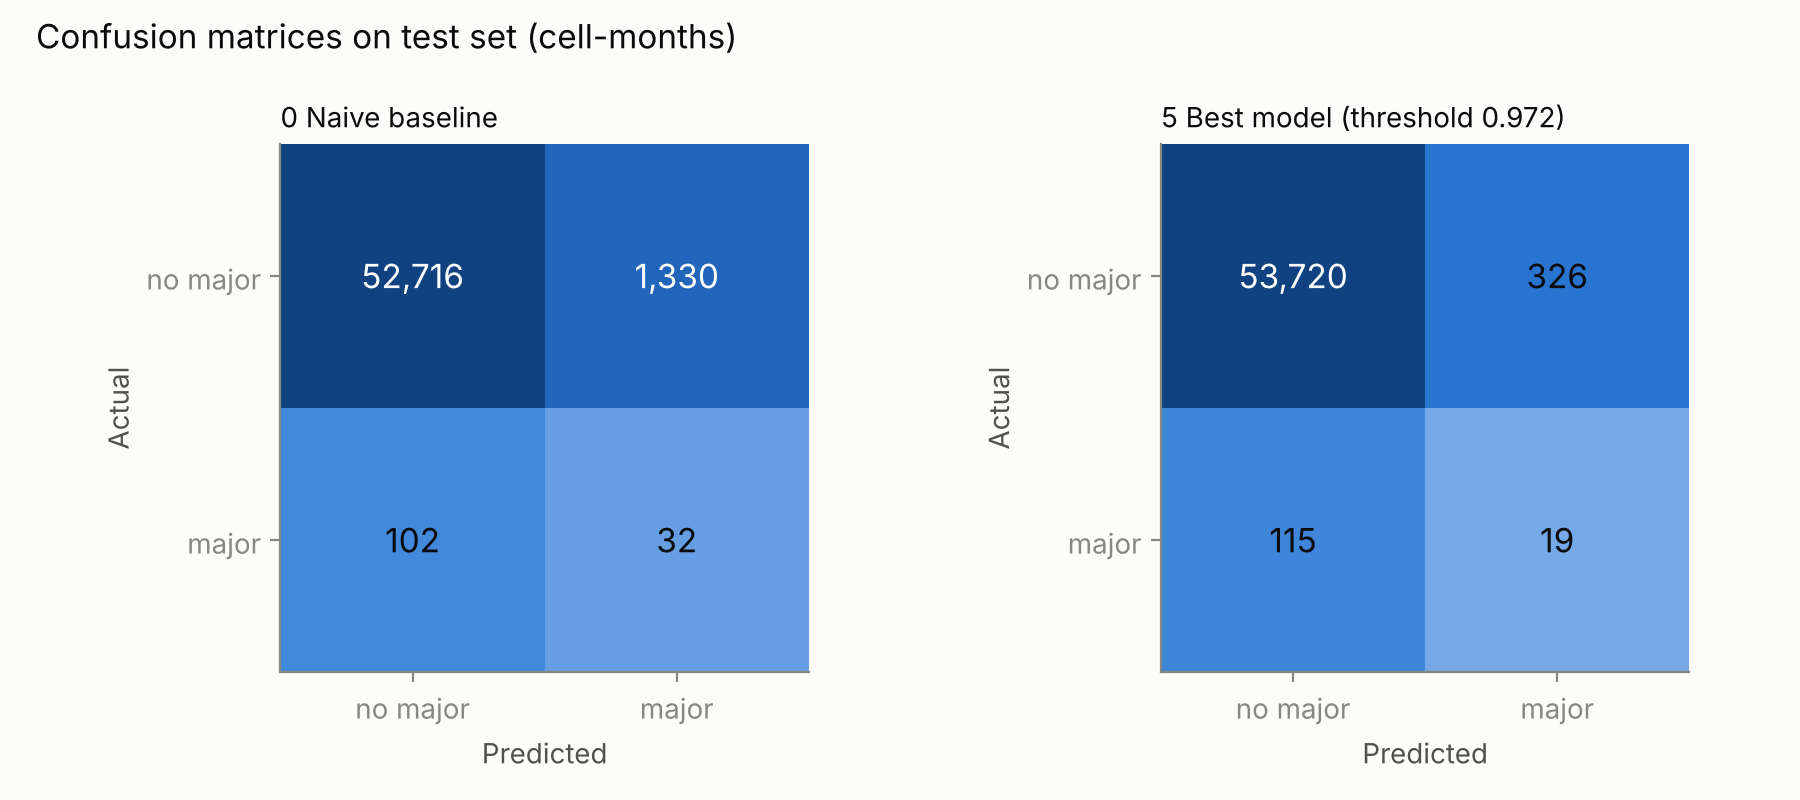
\includegraphics[width=0.49\textwidth]{step9_cm.png}
\caption{ซ้าย: precision-recall curve บนชุด test เส้นประคือการเดาสุ่ม \quad ขวา: confusion matrix ของ baseline และโมเดลที่ดีที่สุด}
\end{figure}

\begin{figure}[H]
\centering
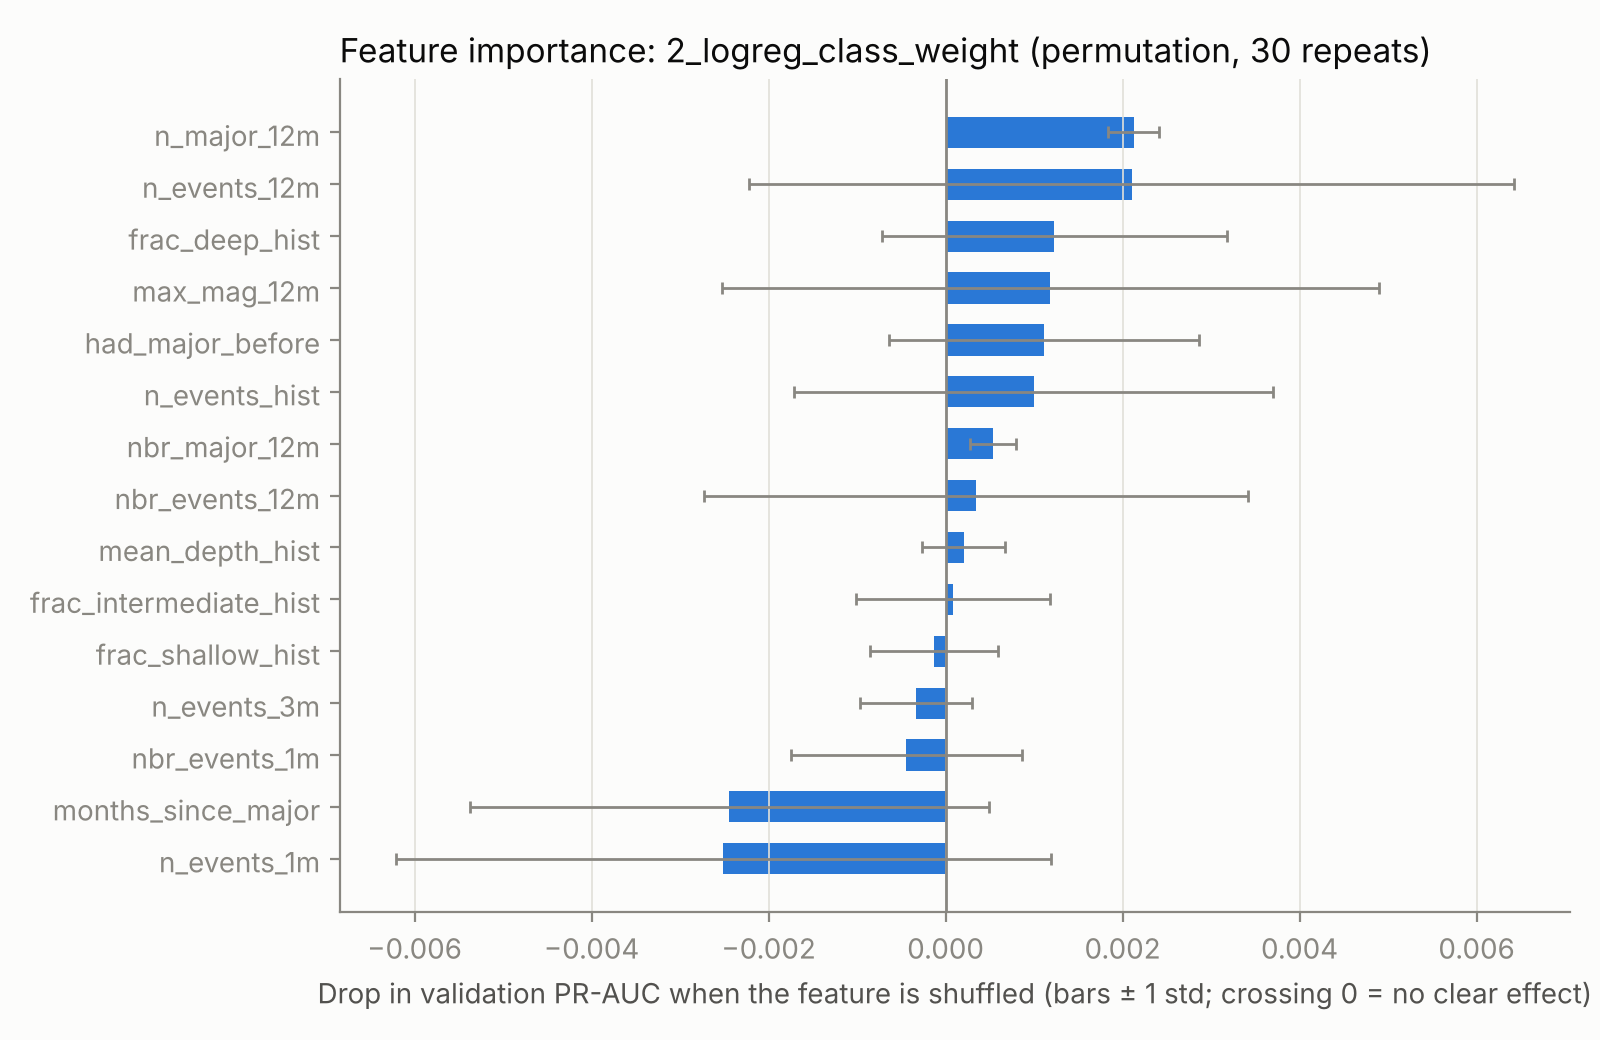
\includegraphics[width=0.7\textwidth]{step9_importance.png}
\caption{Permutation importance บน validation (PR-AUC ที่ลดลงเมื่อสลับค่า feature)}
\end{figure}

%======================================================================
\section{Live Demo}
%======================================================================

เพื่อจำลองข้อมูลสด เรากำหนดจุดเริ่มต้นของช่วงสดเป็น 8 ต.ค. 2026 10:00 UTC
เหตุการณ์ที่เกิดหลังเวลานี้และถูกพบครั้งแรกหลังเวลานี้ (\code{first\_seen\_at}) ถือเป็นข้อมูลสด
แล้วรัน \code{usgs\_fetch.py} 2 ครั้ง

\begin{table}[H]
\centering\small
\resizebox{\textwidth}{!}{%
\begin{tabular}{@{}lrrl@{}}
\toprule
เวลาที่ดึง (UTC) & เหตุการณ์สดใหม่ & เหตุการณ์เก่าที่เพิ่งเข้ามา & เหตุการณ์เก่าสุดที่เพิ่งเข้ามา \\
\midrule
2026-10-08 10:02 & 0 & 1 & 2026-10-08 \\
2026-10-10 12:36 & 69 & 21 & 2026-07-20 \\
\bottomrule
\end{tabular}}
\caption{ผลการดึงข้อมูลสด (\code{results/step10\_fetch\_runs.csv})}
\end{table}

\begin{itemize}
  \item ในช่วง 48.5 ชั่วโมง มีเหตุการณ์ใหม่ 69 ครั้ง (34.2 ครั้งต่อวัน) ใน 24 ช่องตาราง ใหญ่สุดคือ M7.7 ที่ปานามา
  \item การดึงครั้งที่สองได้เหตุการณ์เก่าที่ USGS เพิ่งเพิ่มเข้ามา 21 รายการ เก่าสุดย้อนไปถึง ก.ค. 2026 แสดงว่าแคตตาล็อกเปลี่ยนย้อนหลังจริง และ \code{updatedafter} เก็บได้ครบ
  \item เหตุการณ์ใหม่ถูกส่งเข้าโมเดล Isolation Forest (ชุด B) ที่บันทึกไว้จาก Step 6 ช่อง-สัปดาห์ของ M7.7 ปานามาได้คะแนน 0.677 ต่ำกว่าเกณฑ์ 0.683 จึงไม่ถูก flag เพราะตอนนั้นสัปดาห์ยังไม่จบ จำนวนเหตุการณ์จึงยังไม่ครบ
  \item แผนที่ replay แบบ interactive อยู่ที่ \code{figures/step10\_live\_replay.html}
\end{itemize}

\begin{figure}[H]
\centering
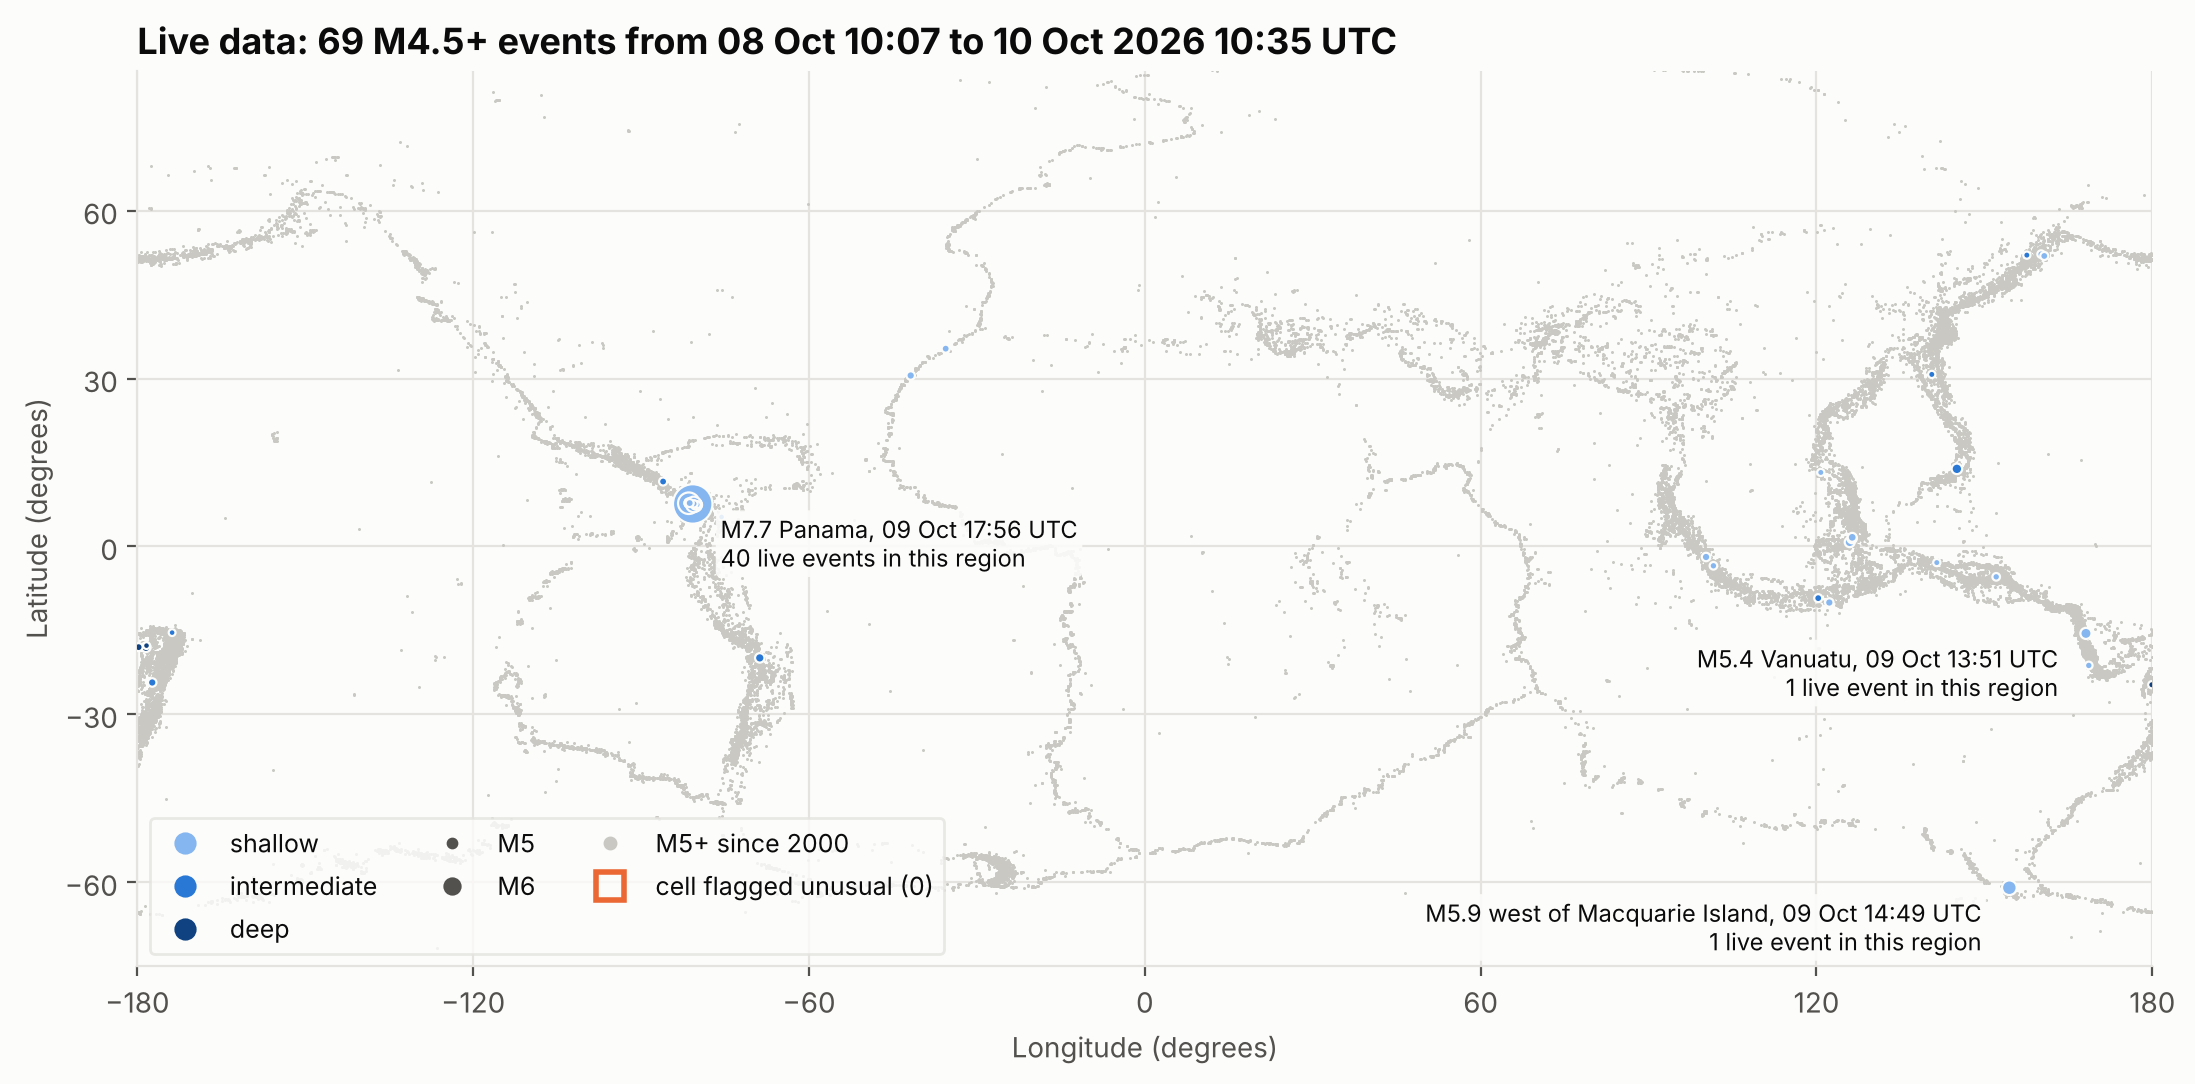
\includegraphics[width=\textwidth]{step10_live_map.png}
\caption{เหตุการณ์ในช่วงข้อมูลสด 8--10 ต.ค. 2026}
\end{figure}

%======================================================================
\section{การประยุกต์ใช้}
%======================================================================

\begin{itemize}
  \item \textbf{ติดตาม aftershock:} ST-DBSCAN แยกกลุ่ม aftershock ออกจากกิจกรรมปกติ ช่วยประเมินว่าลำดับ aftershock ยังดำเนินอยู่หรือสงบแล้ว
  \item \textbf{Dashboard แบบ real-time:} \code{usgs\_fetch.py} ร่วมกับ Isolation Forest flag ช่องตารางที่มีกิจกรรมสูงผิดปกติทันทีที่มีข้อมูลใหม่
  \item \textbf{จัดลำดับพื้นที่เสี่ยง:} โมเดลจำแนกจัดอันดับช่องตารางได้ดีกว่าการเดาสุ่ม 16 เท่า ใช้ช่วยจัดลำดับการตรวจสอบอาคารหรือการกำหนดเบี้ยประกันภัยได้ แต่ใช้เตือนภัยรายเดือนไม่ได้
  \item \textbf{ตรวจคุณภาพแคตตาล็อก:} การตรวจความลึกที่ตั้งไว้ล่วงหน้าและเหตุการณ์ซ้ำ ใช้เป็นขั้นตอนมาตรฐานก่อนวิเคราะห์ข้อมูลแผ่นดินไหวอื่นได้
\end{itemize}

%======================================================================
\section{ข้อจำกัดและงานในอนาคต}
%======================================================================

\begin{itemize}
  \item \textbf{การทำนายแผ่นดินไหวยากโดยธรรมชาติ:} ผลการจำแนกต่ำ (F1 0.079) ไม่ใช่ความล้มเหลวของวิธี แต่สะท้อนว่าประวัติในอดีตบอกได้แค่ว่าพื้นที่ไหนเสี่ยงกว่า ไม่ได้บอกเวลาที่แน่นอน
  \item \textbf{Leakage:} เราป้องกันด้วยการแบ่งตามเวลา, คำนวณค่าปกติจากช่วง train เท่านั้น, ทำ SMOTE และ scaler บน train เท่านั้น, และทดสอบตัดข้อมูลอนาคต ส่วน Isolation Forest แสดงให้เห็นว่าถ้าใส่ขนาดสูงสุด precision จะพองจาก 0.424 เป็น 0.759
  \item \textbf{แคตตาล็อกต่ำกว่า M4.5 ไม่สมบูรณ์:} Mc ทั่วโลกคือ 4.7 ข้อมูลช่วง 4.5--4.7 จึงขาดบางส่วน โดยเฉพาะในพื้นที่ที่มีสถานีวัดน้อยและในปีแรก ๆ
  \item \textbf{ขนาดวัดหลายสเกล:} เราใช้ \code{mag} ตามที่ USGS ให้มาโดยไม่แปลงให้เป็นสเกลเดียวกัน mb ซึ่งเป็นส่วนใหญ่อิ่มตัวที่ขนาดใหญ่
  \item \textbf{ความลึกที่ตั้งไว้ล่วงหน้า:} 46.4\% ของความลึกไม่ใช่ค่าจริง feature ที่ใช้ความลึกจึงมีสัญญาณรบกวน
  \item \textbf{ช่องตารางคงที่:} ช่อง $5^\circ$ ไม่ตรงกับรูปร่างของรอยเลื่อน และพื้นที่จริงของช่องเล็กลงเมื่อเข้าใกล้ขั้วโลก
  \item \textbf{ข้อมูลสดขาดช่วง:} เราไม่ได้รันสคริปต์ตลอดเวลา \code{first\_seen\_at} ของช่วงที่ไม่ได้รันจึงเป็นเวลาที่รันครั้งถัดไป ช่วงข้อมูลสดมีแค่ 48.5 ชั่วโมง
  \item \textbf{งานในอนาคต:} แปลงขนาดให้เป็น Mw, ใช้ช่องตารางที่ปรับตามแนวรอยเลื่อน, เพิ่ม feature จากแบบจำลอง ETAS, และรันข้อมูลสดต่อเนื่องเป็นเวลานานขึ้น
\end{itemize}

%======================================================================
\begin{thebibliography}{99}
\phantomsection
\addcontentsline{toc}{section}{\refname}
%======================================================================
\bibitem{usgs-api} U.S. Geological Survey. \textit{Earthquake Catalog API Documentation (FDSN Event Web Service)}. \url{https://earthquake.usgs.gov/fdsnws/event/1/}

\bibitem{gr1944} Gutenberg, B., \& Richter, C. F. (1944). Frequency of earthquakes in California. \textit{Bulletin of the Seismological Society of America}, 34(4), 185--188.

\bibitem{aki1965} Aki, K. (1965). Maximum likelihood estimate of $b$ in the formula $\log N = a - bM$ and its confidence limits. \textit{Bulletin of the Earthquake Research Institute}, 43, 237--239.

\bibitem{wiemer2000} Wiemer, S., \& Wyss, M. (2000). Minimum magnitude of completeness in earthquake catalogs: Examples from Alaska, the western United States, and Japan. \textit{Bulletin of the Seismological Society of America}, 90(4), 859--869.

\bibitem{woessner2005} Woessner, J., \& Wiemer, S. (2005). Assessing the quality of earthquake catalogues: Estimating the magnitude of completeness and its uncertainty. \textit{Bulletin of the Seismological Society of America}, 95(2), 684--698.

\bibitem{ester1996} Ester, M., Kriegel, H.-P., Sander, J., \& Xu, X. (1996). A density-based algorithm for discovering clusters in large spatial databases with noise. \textit{Proceedings of KDD-96}, 226--231.

\bibitem{birant2007} Birant, D., \& Kut, A. (2007). ST-DBSCAN: An algorithm for clustering spatial--temporal data. \textit{Data \& Knowledge Engineering}, 60(1), 208--221.

\bibitem{satopaa2011} Satopää, V., Albrecht, J., Irwin, D., \& Raghavan, B. (2011). Finding a ``kneedle'' in a haystack: Detecting knee points in system behavior. \textit{ICDCS Workshops}, 166--171.

\bibitem{utsu1995} Utsu, T., Ogata, Y., \& Matsu'ura, R. S. (1995). The centenary of the Omori formula for a decay law of aftershock activity. \textit{Journal of Physics of the Earth}, 43(1), 1--33.

\bibitem{liu2008} Liu, F. T., Ting, K. M., \& Zhou, Z.-H. (2008). Isolation forest. \textit{Proceedings of the 8th IEEE International Conference on Data Mining}, 413--422.

\bibitem{chawla2002} Chawla, N. V., Bowyer, K. W., Hall, L. O., \& Kegelmeyer, W. P. (2002). SMOTE: Synthetic minority over-sampling technique. \textit{Journal of Artificial Intelligence Research}, 16, 321--357.

\bibitem{ke2017} Ke, G., Meng, Q., Finley, T., Wang, T., Chen, W., Ma, W., Ye, Q., \& Liu, T.-Y. (2017). LightGBM: A highly efficient gradient boosting decision tree. \textit{Advances in Neural Information Processing Systems 30}, 3146--3154.

\bibitem{sklearn} Pedregosa, F., et al. (2011). Scikit-learn: Machine learning in Python. \textit{Journal of Machine Learning Research}, 12, 2825--2830.

\bibitem{saito2015} Saito, T., \& Rehmsmeier, M. (2015). The precision-recall plot is more informative than the ROC plot when evaluating binary classifiers on imbalanced datasets. \textit{PLoS ONE}, 10(3), e0118432.
\end{thebibliography}

%======================================================================
\appendix
\section{ภาคผนวก: หน้าที่ของสมาชิก}
%======================================================================

\begin{table}[H]
\centering\small
\begin{tabularx}{\textwidth}{@{}lX@{}}
\toprule
สมาชิก & งานที่ทำ \\
\midrule\relax
ปุณณวิชญ์ คล้ายรักษ์ & ทดลองดึงข้อมูลรอบแรก, แก้ปัญหา timeout ของ \code{usgs\_fetch.py}, Step 3 การเตรียมข้อมูล (\code{02\_preprocess.ipynb}), live demo รุ่นแรก \\\relax
ศรัณย์ ชัยกุลเสรีวงค์ & ออกแบบและเขียน \code{usgs\_fetch.py} และ \code{config.py}, Step 4 EDA, Step 5 ST-DBSCAN, Step 6 Isolation Forest, เอกสารอธิบาย Step 3--6, Step 11 ล็อกผล \\
พีรณัฐ ทัศนวิญญู & Step 7 ตาราง feature และการตรวจ leakage, Step 8 imbalanced classification และการปรับ LightGBM, Step 9 การประเมินผล, Step 10 live demo \\
\bottomrule
\end{tabularx}
\caption{หน้าที่ของสมาชิก (จาก commit ใน GitHub) ให้สมาชิกตรวจและแก้ให้ตรงก่อนส่ง}
\end{table}

\noindent โค้ดและผลลัพธ์ทั้งหมด: \url{https://github.com/tls123qq/Earthquake-project}
\\ ตัวเลขทุกตัวในรายงานนี้คัดมาจาก \code{results/step11\_final\_numbers.md}

\end{document}